\documentclass[a4paper,11pt]{article}
\usepackage{fix-cm}
% --- IMPOSTAZIONI LINGUA E CODIFICA ---
\usepackage[english]{babel}
%\usepackage[utf8]{inputenc}
\usepackage[T1]{fontenc}
\usepackage{lmodern}
% --- FONT ARIAL (Helvetica) ---
\usepackage[scaled]{helvet}
\renewcommand{\familydefault}{\sfdefault}

% --- PACCHETTI UTILI ---
\usepackage{lastpage}
\usepackage{amsmath, amssymb}
\usepackage{graphicx}
\usepackage{booktabs}
\usepackage{hyperref}
\usepackage{enumitem}
\usepackage{float}
\usepackage{subcaption}
\usepackage{geometry}
\usepackage{fancyhdr}
\setlength{\headheight}{13.6pt}
\usepackage{lastpage}
\usepackage{xcolor}
\usepackage{tikz}
\usepackage{adjustbox}
\usetikzlibrary{matrix, positioning, shapes.geometric, arrows.meta, fit, backgrounds, calc, shadows}
\usepackage{appendix}

%\usepackage[title,titletoc]{APPENDICE}

% Comando per cambiare lo stile nelle appendici
\newcommand{\setupappendixstyle}{
    \newpage
    \pagestyle{fancy}
    \fancyhf{} % Pulisce header e footer precedenti
    
    % Configurazione Header Dinamico: solo "Appendice" + Lettera
    \fancyhead[L]{\textbf{\small APPENDICE \thesection}} 
    \fancyhead[R]{\small \textit{Documentazione Integrativa}}
    
    % Footer (manteniamo la numerazione pagine)
    \fancyfoot[C]{\textcolor{BrandGrayMid}{\small Pagina \thepage\ di \pageref{LastPage}}}
    
    % Reset contatori per Figure e Tabelle (es. A.1, B.1)
    \renewcommand{\thefigure}{\thesection.\arabic{figure}}
    \renewcommand{\thetable}{\thesection.\arabic{table}}
}


\tikzset{
  flow/node/.style={
    font=\small,
    align=center,
    rounded corners=3pt,
    draw=BrandGrayDark,
    line width=0.6pt,
    text=BrandTextPrimary,
    fill=SideBarColor,
    minimum height=9mm,
    text width=4.2cm,
    drop shadow={shadow xshift=0.8pt, shadow yshift=-0.8pt, opacity=0.18}
  },
  flow/startstop/.style={
    flow/node,
    fill=BrandPaper,
    draw=BrandAccentRed,
    line width=0.8pt,
    text width=4.2cm
  },
  flow/process/.style={
    flow/node
  },
  flow/data/.style={
    flow/node,
    fill=BrandPaper
  },
  flow/decision/.style={
    font=\small,
    align=center,
    diamond,
    aspect=2.2,
    inner sep=1.2pt,
    draw=BrandAccentRed,
    line width=0.8pt,
    text=BrandTextPrimary,
    fill=BrandPaper,
    drop shadow={shadow xshift=0.8pt, shadow yshift=-0.8pt, opacity=0.18}
  },
  flow/arrow/.style={
    -{Latex[length=2.2mm,width=1.6mm]},
    line width=0.7pt,
    draw=BrandAccentRed
  },
  flow/label/.style={
    font=\scriptsize,
    text=BrandGrayDark,
    fill=white,
    fill opacity=0.85,
    text opacity=1,
    inner sep=1.2pt,
    rounded corners=2pt
  }
}


\geometry{margin=2.5cm, headsep=0.8cm, footskip=1cm}

% --- COLORI DEL NOTEBOOK (Design System) ---
\definecolor{BrandTextPrimary}{HTML}{111111}
\definecolor{BrandAccentRed}{HTML}{222255}
\definecolor{BrandGrayDark}{HTML}{404040}
\definecolor{BrandGrayMid}{HTML}{737373}
\definecolor{BrandPaper}{HTML}{E8E8E6}
\definecolor{SideBarColor}{HTML}{F5F5F5} % Colore sfondo laterale

% --- HEADER E FOOTER (Pagine interne) ---
\pagestyle{fancy}
\fancyhf{}
\fancyhead[L]{\textbf{\small Andrea Palazzo - Analytics • Intelligence • Strategy}}
\fancyhead[R]{\small \textit{Analisi Predittiva Income}}
\fancyfoot[C]{\textcolor{BrandGrayMid}{\small Pagina \thepage\ di \pageref{LastPage}}}
\renewcommand{\headrulewidth}{0.5pt}
\renewcommand{\headrule}{\color{BrandAccentRed}\hrule width\headwidth height\headrulewidth \kern-\headrulewidth}

% --- CONFIGURAZIONE DOCUMENTO ---
\hypersetup{
    colorlinks=true,
    linkcolor=BrandAccentRed,
    urlcolor=BrandAccentRed,
    pdftitle={Analisi e Predizione del Reddito Adult Census Income},
    pdfauthor={Andrea Palazzo}
}

\begin{document}

% --- TITLE PAGE CORPORATE ---
\begin{titlepage}
    \pagestyle{empty} % Nessun header/footer nella copertina
    \begin{tikzpicture}[remember picture, overlay]
        
        % 1. Fascia laterale sinistra (Grigio chiaro)
        \fill[SideBarColor] (current page.north west) rectangle ($(current page.south west) + (6cm, 0)$);
        
        % 2. Linea accento verticale (Rosso brand)
        \fill[BrandAccentRed] ($(current page.north west) + (6cm, 0)$) rectangle ($(current page.south west) + (6.15cm, 0)$);
        
        % 3. LOGO (Sostituisci 'logo.png' con il nome del tuo file)
        % Posizionato in alto a sinistra nella fascia laterale
        \node[anchor=north west, inner sep=0] at ($(current page.north west) + (1cm, -1.5cm)$) {
            % Se non hai il file, decommenta la riga sotto per vedere un placeholder
            \includegraphics[width=4cm]{figure_vecchie/logo.png} 
            
            % Placeholder temporaneo se non hai il PNG pronto (puoi rimuoverlo)
            %\begin{tikzpicture}
            %   \node[fill=white, draw=BrandGrayDark, text width=3.5cm, align=center, % minimum height=3.5cm] 
            %   {\Huge\bfseries\color{BrandAccentRed}$\alpha$};
            %\end{tikzpicture}
        };

        % 4. Info Autore nella fascia laterale (in basso)
        \node[anchor=south west, align=left, text width=4.5cm] at ($(current page.south west) + (1cm, 2cm)$) {
            \color{BrandGrayDark}
            \small \textbf{}\\[0.1cm]
            \Large \textbf{Andrea Palazzo}\\[0.1cm]
            \small Data Manager Student
            \vspace{0.5cm}
            
            \small \textbf{}\\[0.1cm]
            %\today
            \vspace{0.5cm}
            
           
        };

        % 5. Area Titolo (Parte destra bianca)
        \node[anchor=north west, align=left, text width=12cm] at ($(current page.north west) + (7.5cm, -6cm)$) {
            \color{BrandAccentRed}\sffamily\bfseries\small REPORT TECNICO
            \vspace{0.3cm}
            
            \color{BrandTextPrimary}\sffamily\bfseries\fontsize{35}{40}\selectfont
            Analisi e Predizione\\
            del Reddito
            \vspace{0.5cm}
            
            \color{BrandGrayDark}\sffamily\huge\textit{Adult Census Income Dataset}
            \vspace{1.5cm}
            
            \color{BrandGrayMid}\normalsize
            Studio applicativo di machine learning su dati censuari per la previsione del reddito.
        };

        % 6. Elemento grafico decorativo in basso a destra
        \node[anchor=south east] at ($(current page.south east) + (-1cm, 1cm)$) {
             \fontsize{60}{70}\selectfont\color{BrandPaper}\textbf{BI}
        };

    \end{tikzpicture}
\end{titlepage}

\newpage
\pagestyle{fancy}


%=====================================================================================================
%=====================================================================================================
% abstract
%=====================================================================================================
\begin{abstract}
\noindent Questo lavoro affronta un problema di classificazione binaria sul dataset \textit{Adult Census Income}, con l’obiettivo di predire se il reddito annuale di un individuo superi la soglia dei 50.000 dollari.
L’analisi evidenzia un marcato sbilanciamento di classe e la presenza di valori mancanti codificati come \texttt{?}, gestiti tramite conversione e rimozione delle osservazioni incomplete; inoltre, la variabile \texttt{fnlwgt} viene esclusa per il ridotto potere discriminante e la variabile \texttt{native.country} viene ricondotta a una codifica più robusta a bassa cardinalità.
Dopo una fase di esplorazione e definizione della pipeline di preprocessing, vengono confrontati diversi algoritmi supervisionati mediante validazione incrociata, selezionando i modelli di gradient boosting come candidati principali per l’ottimizzazione degli iperparametri.
Il modello finale, un XGBoost ottimizzato, ottiene sul test set indipendente un’accuracy pari a 0.8540 e un F1-score pari a 0.7330, con ROC-AUC pari a 0.931, confermando buone capacità di generalizzazione e un compromesso efficace tra precision e recall in presenza di classi sbilanciate.
\end{abstract}

\newpage
\tableofcontents
\newpage


%=====================================================================================================
%=====================================================================================================
% corpo del documento
%=====================================================================================================







\section{Introduzione}

Il dataset \textit{Adult Census Income} rappresenta un benchmark consolidato nel machine learning per lo studio di problemi di classificazione binaria su dati tabellari eterogenei. 
L’obiettivo di questo lavoro è la previsione del reddito individuale, formalizzata come la classificazione della variabile target \texttt{income} rispetto al superamento o meno della soglia annuale di 50.000 dollari. 
Il contesto applicativo presenta complessità tipiche degli scenari reali, tra cui la coesistenza di variabili categoriche e numeriche e lo sbilanciamento tra le classi della variabile target. 

\subsection{Obiettivo e impostazione del problema}
Il progetto mira a costruire un flusso di lavoro completo e riproducibile che includa analisi esplorativa, pulizia dei dati, preprocessing, feature engineering e valutazione comparativa di modelli supervisionati. 
In presenza di classi sbilanciate, l’analisi pone particolare attenzione alla scelta di metriche di valutazione robuste e all’interpretazione degli errori di classificazione sulla classe minoritaria. 
L’output atteso è un modello finale con buone capacità di generalizzazione, valutato su un insieme di test indipendente e discusso anche attraverso analisi diagnostiche e strumenti di interpretabilità. 

\subsection{Sfide principali}
L’analisi del dataset evidenzia che eventuali valori mancanti possono essere codificati in forma non standard (ad esempio tramite il placeholder \texttt{?}), rendendo necessarie procedure esplicite di individuazione e trattamento. 
Inoltre, lo sbilanciamento della variabile target implica che metriche come la sola accuracy possano fornire una rappresentazione incompleta delle prestazioni, richiedendo un’analisi centrata anche su precision, recall, F1-score e curve di valutazione appropriate. 
Infine, la presenza di variabili ad alta cardinalità e la natura mista delle feature (categoriche e numeriche) richiedono scelte metodologiche coerenti nella progettazione della pipeline di preprocessing. 

\begin{figure}[H]
    \centering
    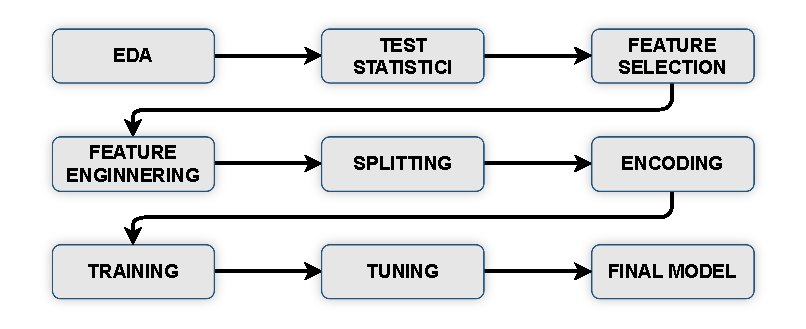
\includegraphics[width=1\textwidth]{fc_p.pdf}
    \caption{Pipeline metodologica del progetto. Il diagramma illustra il flusso di lavoro completo, partendo dalla fase di Analisi Esplorativa dei Dati (EDA) e Preprocessing, passando per la Feature Engineering e selezione delle variabili, fino all'addestramento, validazione e definizione del modello di Machine Learning finale.}
    \label{fig:ml_pipeline}
\end{figure}


\newpage
\section{Storia e Origine del Dataset}

I dati originali provengono dal database del censimento degli Stati Uniti del 1994. L'estrazione fu curata da Barry Becker in collaborazione con Ronny Kohavi (all'epoca presso la Data Mining and Visualization di Silicon Graphics) e donata all'\textit{UCI Machine Learning Repository} il 30 aprile 1996.

\subsection{Criteri di Costruzione e Filtraggio del Dataset}

Un aspetto cruciale per comprendere la struttura attuale del dataset riguarda i criteri di filtraggio utilizzati dagli autori originali. Per ottenere dati coerenti e utilizzabili a fini di analisi, Becker e Kohavi applicarono delle query specifiche al database grezzo. Tali criteri spiegano l'origine delle attuali variabili e la selezione delle osservazioni presenti nel dataset finale:

\begin{itemize}
\item \textbf{AAGE > 16}: Esclusione dei minorenni; nel dataset finale questa informazione è rappresentata dalla variabile {age}.
\item \textbf{HRSWK > 0}: Esclusione degli individui non occupati; corrisponde alla variabile {hours-per-week}.
\item \textbf{AFNLWGT > 1}: \textit{Final weight}, peso statistico utilizzato dal Census Bureau per garantire la rappresentatività del campione; corrisponde alla variabile {fnlwgt}.
\item \textbf{AGI > 100}: \textit{Adjusted Gross Income}, utilizzato per filtrare redditi non significativi e per la costruzione della variabile target.
\end{itemize}

\noindent
Il risultato di questo processo è un dataset composto da 48.842 osservazioni e 14 variabili esplicative, comprendenti attributi demografici, educativi e occupazionali.

\newpage
\section{Ambiente di Sviluppo e Strumenti}

L'analisi è stata condotta utilizzando il linguaggio Python (versione 3.13.2) all'interno di un ambiente Jupyter Notebook. Al fine di garantire la riproducibilità dell'analisi e l'efficienza computazionale, sono state adottate librerie consolidate nell'ecosistema della data science, ciascuna con un ruolo specifico all'interno del flusso di lavoro:

\begin{itemize}
    \item \textbf{Data Manipulation:} {pandas} e {numpy} per la gestione strutturata dei dati e le operazioni vettoriali.
    \item \textbf{Visualizzazione:} {matplotlib} e {seaborn} per la produzione di grafici statici ad alta risoluzione, integrati da {plotly} per l'esplorazione interattiva dei dati.
    \item \textbf{Machine Learning:} Il framework {scikit-learn} ha fornito la base per le fasi di preprocessing, modellazione e valutazione delle prestazioni.
    \item \textbf{Gradient Boosting Avanzato:} Sono state integrate librerie specializzate quali {XGBoost}, {LightGBM} e {CatBoost} per il confronto di algoritmi allo stato dell’arte su dati tabellari.
\end{itemize}

\newpage
\section{Descrizione del Dataset}

\subsection{Origine e Acquisizione dei Dati}
L'analisi è stata condotta sul dataset \textit{Adult Census Income}, acquisito tramite il repository ufficiale UCI Machine Learning Repository (tramite KaggleHub). Si precisa che il dataset utilizzato non corrisponde esattamente alla versione grezza del censimento del 1994, ma a una versione preprocessata e consolidata resa disponibile dal repository UCI.

\subsection{Struttura e Tipologia delle Variabili}
Il dataset presenta una struttura eterogenea, composta da variabili sia categoriche che numeriche. In particolare:
\begin{itemize}
    \item \textbf{Variabili Categoriche (8):} {workclass}, {education}, {marital.status}, {occupation}, {relationship}, {race}, {sex} e {native.country}.
    \item \textbf{Variabili Numeriche (6):} {age}, {fnlwgt}, {education.num}, {capital.gain}, {capital.loss} e {hours.per.week}.
\end{itemize}

\noindent Il dataset contiene inizialmente 32.561 osservazioni, ciascuna descritta da 14 variabili esplicative, oltre la variabile target {income} di tipo categorico binario e indica se il reddito annuale dell’individuo supera o meno la soglia dei 50.000 dollari.
\noindent
Le caratteristiche strutturali e la distribuzione delle variabili verranno analizzate in dettaglio nella successiva fase di analisi esplorativa dei dati.


\newpage
\newpage
\section{Analisi Esplorativa dei Dati (EDA)}

L'analisi si è concentrata su:
\begin{enumerate}[label=(\roman*)]
    \item distribuzione della variabile target e sbilanciamento;
    \item presenza e struttura dei valori mancanti;
    \item evidenze preliminari di separabilità tra classi tramite feature categoriche e numeriche;
    \item verifica di possibili fenomeni di multicollinearità sulle variabili numeriche.
\end{enumerate}

\subsubsection{Distribuzione della variabile target e sbilanciamento}
La variabile target \texttt{income} presenta una distribuzione fortemente asimmetrica, con una classe maggioritaria (\(\leq 50K\)) pari a circa il 76\% delle osservazioni e una classe minoritaria (\(>50K\)) pari a circa il 24\%. 
Questo rapporto (circa 3:1) configura un tipico scenario di \textit{imbalanced classification}, in cui l’accuracy può risultare fuorviante se utilizzata come unico indicatore di performance. 
Di conseguenza, nelle fasi successive vengono privilegiate metriche robuste allo sbilanciamento (ad es.\ Precision, Recall, F1-score e ROC-AUC) e viene posta attenzione specifica alla capacità di riconoscere correttamente la classe minoritaria. 

\subsection{Valori mancanti e pattern di mancanza}
Un primo controllo visivo non evidenzia valori nulli, ma un’analisi più approfondita mostra che i dati mancanti sono codificati tramite il placeholder \texttt{?} anziché come \texttt{NaN}. 
Dopo la conversione del placeholder, i missing risultano concentrati soprattutto in \texttt{occupation} (circa 5.66\%), \texttt{workclass} (circa 5.64\%) e \texttt{native.country} (circa 1.79\%). 
L’EDA evidenzia inoltre un pattern strutturale di mancanza congiunta tra \texttt{workclass} e \texttt{occupation}; data la difficoltà di imputare valori plausibili senza introdurre distorsioni, si è deciso di rimuovere le osservazioni incomplete (\textit{listwise deletion}), con una riduzione complessiva di circa il 7.44\% del dataset. 

\subsection{Evidenze preliminari sulle feature}
Le analisi descrittive sulle variabili categoriche mostrano relazioni informative con il target per variabili socio-demografiche e lavorative (ad es.\ \texttt{education}, \texttt{marital.status}, \texttt{occupation}, \texttt{relationship}), suggerendo che tali attributi contribuiscano alla separazione tra classi. 
Per la variabile \texttt{sex} emerge un gap marcato: la probabilità di reddito \(>50K\) risulta sensibilmente più alta per gli uomini rispetto alle donne nel campione osservato. 
Per le variabili numeriche, l’analisi evidenzia che \texttt{age}, \texttt{education.num} e \texttt{hours.per.week} tendono ad assumere valori più elevati nella classe \(>50K\), mentre \texttt{capital.gain} e \texttt{capital.loss} presentano una forte \textit{zero-inflation} (molti zeri e pochi valori estremi), indicando eventi rari ma potenzialmente molto informativi quando presenti. 
La variabile \texttt{fnlwgt} mostra invece distribuzioni molto simili tra le due classi, suggerendo un potere discriminante limitato e motivando una successiva valutazione critica del suo utilizzo nel modello. 

\subsection{Correlazioni e multicollinearità}
Come verifica finale dell’EDA, è stata calcolata la matrice di correlazione di Pearson per le variabili numeriche, con l’obiettivo di identificare eventuali relazioni lineari forti e ridondanze informative. 
Dalla matrice non emergono coppie con correlazione elevata oltre le soglie tipicamente considerate critiche (ad es.\ \(r>0.85\)), suggerendo l’assenza di multicollinearità severa tra le feature numeriche. 
Nel complesso, le evidenze dell’EDA guidano le decisioni di preprocessing (gestione missing, trasformazioni e codifiche) e anticipano le feature più promettenti per la fase di modellazione e selezione del modello. 

\newpage
\section{Feature Selection e Inferenza Statistica}

Dopo la fase di EDA, è stata condotta una fase di inferenza statistica con l’obiettivo di validare quantitativamente le evidenze descrittive e selezionare le feature più informative rispetto alla variabile target (\(\leq 50K\) vs \(>50K\)). 
A differenza dell’EDA, che fornisce indicazioni qualitative e visuali, questa fase si basa su test formali di ipotesi affiancati da misure di \textit{effect size}, così da distinguere tra semplice significatività statistica e reale rilevanza predittiva. 

\subsection{Criteri decisionali e soglie operative}
La selezione delle feature è stata guidata da soglie definite \textit{a priori} per rendere il processo riproducibile. In particolare:

\begin{enumerate}[label=(\roman*)]
    \item \textbf{Gestione dei valori mancanti:} le variabili con una quota di \textit{missing} elevata vengono segnalate come critiche (soglia operativa 10\%);
    \item \textbf{Analisi della varianza:} le \textit{feature} a varianza nulla (costanti) sono candidate alla rimozione immediata;
    \item \textbf{Monitoraggio della ridondanza:} per le \textit{feature} numeriche viene verificata la multicollinearità tramite la matrice di correlazione (soglia di attenzione tipica $r > 0.85$);
    \item \textbf{Valutazione della significatività:} poiché in dataset numerosi i $p$-value tendono a essere sempre significativi, la decisione viene guidata dalla grandezza dell'effetto (Cramér's $V$ per le variabili categoriche e Cohen's $d$ per quelle numeriche).
\end{enumerate}


\subsection{Variabili categoriche: test \(\chi^2\) e Cramér’s V}
Per ogni feature categorica è stato applicato un test \(\chi^2\) di indipendenza tra feature e target (H0: indipendenza; H1: associazione). 
Alla significatività è stata affiancata la misura di associazione Cramér’s V, così da quantificare l’intensità della relazione. 
I risultati mostrano che \texttt{relationship} e \texttt{marital.status} sono le variabili con associazione più elevata (Cramér’s V circa 0.45), seguite da \texttt{education} (circa 0.37) e \texttt{occupation} (circa 0.35), mentre \texttt{race} e \texttt{native.country} risultano statisticamente significative ma con effect size debole (circa 0.10). 

\subsection{Variabili numeriche: Mann--Whitney U e Cohen’s \(d\)}
Dato che l’EDA evidenzia distribuzioni non gaussiane e forte asimmetria per alcune variabili, è stato adottato un test non parametrico di Mann--Whitney U per confrontare le distribuzioni tra le due classi. 
Come misura standardizzata della separazione tra gruppi è stato calcolato Cohen’s \(d\), utile per ordinare le feature in base alla capacità discriminante. 
Tra le variabili numeriche, \texttt{education.num} emerge come la più discriminante (Cohen’s \(d\) circa 0.83), seguita da \texttt{age} e \texttt{hours.per.week} (entrambe circa 0.55), mentre \texttt{fnlwgt} risulta non informativa (p-value circa 0.053 e \(d\) circa 0.02), motivandone l’esclusione. 

\subsection{Output della selezione}
Combinando significatività statistica ed effect size, le feature prioritarie identificate includono \texttt{age}, \texttt{education.num}, \texttt{hours.per.week} e, tra le categoriche, \texttt{relationship}, \texttt{marital.status} e \texttt{occupation}. 
Le variabili con contributo potenzialmente utile ma da validare in modellazione includono \texttt{sex}, \texttt{workclass}, \texttt{capital.gain} e \texttt{capital.loss}, anche in considerazione della forte asimmetria e della natura “evento raro” delle ultime due. 
La variabile \texttt{fnlwgt}, priva di potere discriminante, viene candidata alla rimozione per ridurre dimensionalità senza perdita informativa rilevante. 

\newpage
\section{Partizionamento dei Dati e Trasformazione delle Feature}

Prima dell'addestramento è stata definita una procedura standardizzata per:

\begin{enumerate}[label=(\roman*)]
    \item \textbf{Preparazione del target:} codifica della variabile dipendente in formato binario ($0$ e $1$) per i classificatori;
    \item \textbf{Trasformazione delle feature:} conversione delle variabili categoriche e numeriche in un formato adatto ai modelli supervisionati (tramite \textit{encoding} e \textit{scaling});
    \item \textbf{Data splitting:} suddivisione del dataset in \textit{training} e \textit{test set} per stimare correttamente la capacità di generalizzazione del modello su dati non visti.
\end{enumerate}


\subsection{Preparazione del target}
La variabile target \texttt{income}, inizialmente rappresentata come stringa, è stata ripulita da eventuali spazi e successivamente codificata in forma binaria. 
È stata adottata la mappatura \(0 \rightarrow \leq 50K\) e \(1 \rightarrow >50K\), seguita da un controllo di qualità per verificare l’assenza di valori non mappati. 

\subsection{Trasformazione delle feature}
Sulla base delle evidenze emerse nelle fasi precedenti, è stata effettuata una riduzione della dimensionalità rimuovendo la variabile \texttt{fnlwgt} (\textit{Final Weight}), in quanto interpretabile come peso campionario amministrativo e con potere discriminante trascurabile rispetto al target. 
Per mitigare i problemi legati all’alta cardinalità, è stata inoltre trasformata la variabile \texttt{native.country} (inizialmente con molte categorie) in una rappresentazione più robusta, aggregando le modalità in due macro-categorie: \texttt{USA} e \texttt{Other}. 
Questa scelta riduce la frammentazione informativa e limita il rischio di pattern spurii su categorie rare, mantenendo al contempo un’informazione geografica essenziale e gestibile in fase di modellazione. 

\subsection{Strategia di split e riproducibilità}
Il dataset risultante è stato suddiviso in Training set e Test set con una ripartizione 80/20, utilizzando campionamento stratificato sulla variabile target per preservare la proporzione tra classi nei due sottoinsiemi. 
Per garantire riproducibilità sperimentale, lo split è stato eseguito fissando \texttt{random\_state = 42}. 
Nell’impostazione riportata, il training set è composto da 24.111 osservazioni ed è impiegato per addestramento e validazione, mentre il test set è composto da 6.028 osservazioni ed è mantenuto isolato per la valutazione finale. 


\newpage
\section{Modellazione e Benchmark dei Modelli}

Una volta completate le fasi di preprocessing e feature engineering, è stata avviata una procedura di modellazione supervisionata finalizzata a confrontare algoritmi eterogenei e selezionare i candidati più promettenti per l’ottimizzazione. 

\subsection{Protocollo di valutazione}
Il confronto tra i modelli è stato condotto tramite validazione incrociata stratificata (\textit{k}-fold), preservando la distribuzione sbilanciata della variabile target nei vari fold. 
La metrica di riferimento primaria è stata l’F1-score, scelta per il suo equilibrio tra precision e recall in problemi di classificazione binaria con classi sbilanciate. 
Oltre alla performance predittiva, sono stati monitorati anche i tempi di addestramento, così da valutare il compromesso tra qualità e costo computazionale. 

\subsection{Screening iniziale dei modelli}
Sono stati valutati modelli appartenenti a diverse famiglie (lineari, metodi basati su distanza/probabilità, alberi ed ensemble, boosting classico/moderno e reti neurali), con l’obiettivo di ottenere un primo ranking comparativo. 
Il benchmark ha evidenziato una superiorità dei modelli di boosting, in particolare quelli basati su gradient boosting moderno. 
I migliori risultati medi di F1-score in cross-validation sono stati ottenuti da \texttt{LightGBM}, \texttt{CatBoost}, \texttt{Hist Gradient Boosting}, \texttt{XGBoost} e \texttt{Gradient Boosting}, con valori compresi tra 0.68 e 0.72. 
Sulla base di queste evidenze, tali modelli sono stati selezionati come candidati per la fase di ottimizzazione degli iperparametri. 

\newpage
\section{Ottimizzazione degli Iperparametri e Selezione del Modello Finale}

\subsection{Strategia di ottimizzazione}
Per ciascun modello candidato è stata condotta un’ottimizzazione degli iperparametri tramite \textit{Randomized Search}, così da esplorare in modo efficiente lo spazio dei parametri evitando il costo di una ricerca esaustiva. 
La funzione obiettivo è rimasta l’F1-score medio in cross-validation, garantendo coerenza metodologica con la fase di benchmark. 

\subsection{Risultati del tuning e scelta del candidato}
L’ottimizzazione ha prodotto miglioramenti marginali ma consistenti rispetto alle versioni base. 
In particolare, \texttt{LightGBM (Tuned)} ha raggiunto la miglior performance complessiva con un F1-score medio pari a 0.718, mentre \texttt{Hist Gradient Boosting (Tuned)} e \texttt{XGBoost (Tuned)} hanno ottenuto risultati molto simili (F1 $\approx 0.716$). 
Alla luce del ranking in cross-validation, \texttt{LightGBM (Tuned)} è stato selezionato come modello finale candidato alla valutazione su test set indipendente. 

\subsection{Valutazione sul test set (hold-out)}
Il modello selezionato è stato valutato su un test set indipendente, ottenendo: \textbf{Accuracy} 0.875, \textbf{F1-score} 0.732, \textbf{AUC-ROC} 0.932, \textbf{Average Precision} 0.844 e \textbf{Brier Score} 0.087. 
L’analisi della matrice di confusione evidenzia un buon compromesso sulla classe minoritaria (\(>50K\)), con \textit{recall} pari a 0.68 e \textit{precision} pari a 0.79 per tale classe. 
Il confronto tra performance su training set e test set mostra un gap contenuto (circa 0.015 in accuracy), suggerendo un rischio di overfitting limitato. 

\newpage
\section{Analisi del Modello Finale}

\subsection{Selezione del Modello}

Come discusso nella sezione precedente, i risultati della fase di benchmarking e tuning sono stati sintetizzati in una classifica unica che include sia i modelli base sia le rispettive versioni ottimizzate.  
Sulla base dell’F1-score medio in cross-validation, il modello selezionato come migliore compromesso tra performance, stabilità ed efficienza computazionale è risultato essere {LightGBM ottimizzato}.

\subsection{Valutazione Finale su Test Set}

Il modello selezionato è stato valutato su un test set completamente indipendente, mai utilizzato durante le fasi di addestramento, selezione o ottimizzazione degli iperparametri.  
Questa valutazione fornisce una stima realistica delle prestazioni attese in uno scenario operativo reale.

Le prestazioni ottenute sono:
\begin{itemize}
    \item \textbf{Accuracy}: 0.8749
    \item \textbf{F1-score}: 0.7315
    \item \textbf{AUC-ROC}: 0.932
\end{itemize}

\noindent
L’analisi della matrice di confusione evidenzia un buon compromesso tra precisione e capacità di individuare correttamente la classe minoritaria ($>50K$), confermando la validità della scelta della metrica F1-score come criterio principale di selezione.

\subsection{Analisi della Generalizzazione}

Il confronto tra le prestazioni ottenute sul training set e sul test set mostra uno scostamento contenuto (gap inferiore a 0.02 in accuracy), indicando un rischio di overfitting basso.  
Questo risultato suggerisce che il modello abbia appreso pattern generalizzabili piuttosto che memorizzare specificità del campione di addestramento. La stabilità delle performance osservata anche negli altri modelli di boosting conferma l’efficacia delle scelte di preprocessing, selezione delle feature e regolarizzazione implicita adottate nel processo di modellazione.

\paragraph{Osservazioni metodologiche}
\begin{itemize}
    \item L’uso selettivo dello scaling esclusivamente per i modelli sensibili alla scala ha permesso un confronto più equo tra algoritmi eterogenei.
    \item La validazione incrociata a 3 fold rappresenta un compromesso tra affidabilità della stima e costo computazionale; un numero maggiore di fold potrebbe ridurre ulteriormente la varianza della stima.
    \item La scelta di limitare il tuning ai modelli migliori emersi dal benchmark iniziale ha consentito un utilizzo efficiente delle risorse computazionali, mantenendo al contempo un approccio rigoroso.
\end{itemize}

\newpage
\section{Conclusioni}

In questo lavoro è stato affrontato il problema della previsione del reddito individuale utilizzando il dataset \textit{Adult Census Income}, seguendo un flusso metodologico strutturato che va dall’analisi esplorativa dei dati fino alla selezione di un modello predittivo finale.

\noindent
I risultati mostrano come i modelli di gradient boosting moderno, in particolare {LightGBM}, siano in grado di catturare efficacemente le relazioni non lineari presenti nei dati tabellari eterogenei, ottenendo prestazioni elevate e stabili anche in presenza di classi sbilanciate.

\noindent
Tra i principali limiti del lavoro si segnala l’utilizzo di una singola metrica di selezione primaria e una validazione incrociata con un numero limitato di fold. Inoltre, il dataset analizzato presenta una forte omogeneità geografica, che potrebbe limitare la generalizzabilità dei risultati a contesti differenti.





\newpage
\begin{appendices}
    \setupappendixstyle
    % Reset dei contatori per l'appendice
\setcounter{figure}{0}
\renewcommand{\thefigure}{A.\arabic{figure}}
\setcounter{table}{0}
\renewcommand{\thetable}{A.\arabic{table}}


\section{Analisi Esplorativa dei Dati (EDA)}
\label{app:eda}

Questa appendice documenta la fase di esplorazione preliminare del dataset, fornendo evidenze quantitative della struttura distributiva, della qualità dei dati e dei pattern bivariati che guidano le successive decisioni metodologiche. L'EDA rappresenta un passaggio critico per identificare anomalie, valutare la necessità di trasformazioni e formulare ipotesi sui meccanismi generativi sottostanti.


\noindent La struttura eterogenea delle feature rispecchia la natura multidimensionale dei dati censuari: attributi demografici (age, sex, race, native.country), socio-economici (education, marital.status, relationship) e occupazionali (workclass, occupation, hours.per.week), oltre a proxy economici (capital.gain, capital.loss, fnlwgt).

\subsection{Analisi della Variabile Target: Distribuzione e Sbilanciamento}

\subsubsection{Distribuzione marginale delle classi}

La variabile target \texttt{income} è una variabile binaria nominale. (Figura \ref{fig:bilanciamenti_classe.png}).

\begin{figure}[H]
    \centering
    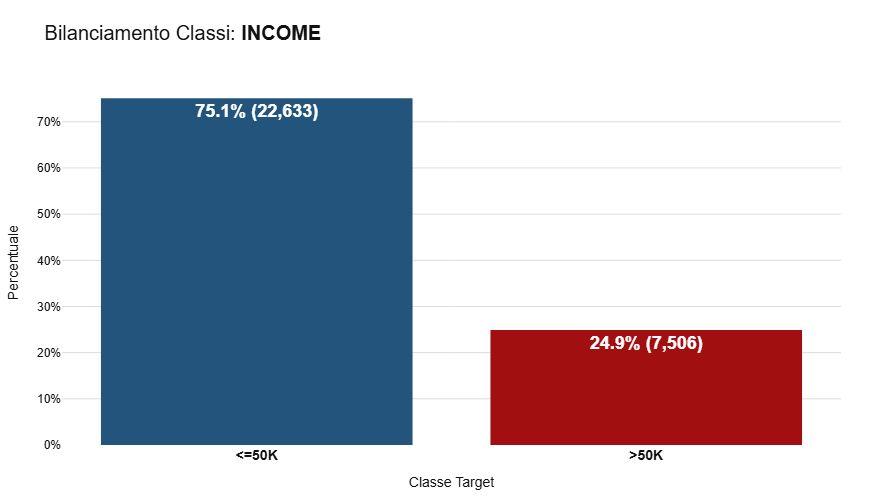
\includegraphics[width=0.75\linewidth]{figures/bilanciamenti_classe.png}
    \caption{\textbf{Distribuzione assoluta e relativa della variabile target} \texttt{income}. Il rapporto approssimativo è di 3:1.}
    \label{fig:bilanciamenti_classe.png}
\end{figure}

\noindent
Il rapporto di sbilanciamento pari a 3.15:1 ($\approx 24.1\% / 75.8\%$) ha importanti implicazioni:

\begin{enumerate}
    \item \textbf{Inadeguatezza dell'Accuracy:} Un classificatore dummy potrebbe predire sempre la classe maggioritaria, risultando però completamente inutile dal punto di vista predittivo.
    
    \item \textbf{Bias verso la classe maggioritaria:} Algoritmi di classificazione standard tendono a privilegiare il riconoscimento della classe dominante, specialmente se non opportunamente regolati. È pertanto necessario adottare metriche robuste (F1-score, ROC-AUC, Average Precision) e strategie di bilanciamento.
    
    \item \textbf{Insufficienza campionaria della classe minority:} Con soli 7.841 esempi positivi, il test set conterrà abbastanza osservazioni di classe minoritaria, fornendo stime di performance con varianza relativamente elevata. Sarà rilevante valutare intervalli di confidenza delle metriche.
    
    \item \textbf{Selezione della soglia decisionale:} La probabilità \textit{a priori} della classe minoritaria è pari a 0.241. Modelli di regressione logistica e probabilistici potranno essere calibrati per utilizzare questa soglia invece della soglia standard di 0.5, migliorando il compromesso Precision-Recall.
\end{enumerate}

\subsection{Analisi dei Valori Mancanti: Rilevamento, Quantificazione e Pattern}

\subsubsection{Decodifica e rilevamento dei placeholder}

Un primo controllo con i comandi pandas standard (\texttt{df.isnull().sum()}) non rivelava alcun valore \texttt{NaN}. Un'ispezione manuale di un sottoinsieme di record rivelò che i dati mancanti erano rappresentati dal token \texttt{?}.

La procedura di bonifica è stata la seguente:
\begin{enumerate}
    \item Sostituzione globale: \texttt{df.replace('?', np.nan, inplace=True)}
    \item Conversione esplicita a NaN per tutte le colonne categoriche
    \item Controllo post-conversione per validare l'assenza di artefatti
\end{enumerate}

\noindent
Tale approccio garantisce coerenza con i standard pandas e consente l'uso di metodi nativi per la gestione dei missing.

\subsubsection{Quantificazione per variabile}

La Tabella \ref{tab:missing} riporta il quadro completo della mancanza dati post-decodifica:

\begin{table}[H]
    \centering
    \begin{tabular}{lrr}
        \toprule
        \textbf{Variabile} & \textbf{Valori Mancanti} & \textbf{Percentuale (\%)} \\
        \midrule
        occupation & 1.843 & 5.66 \\
        workclass & 1.836 & 5.64 \\
        native.country & 583 & 1.79 \\
        \bottomrule
    \end{tabular}
    \caption{Riepilogo delle variabili con valori mancanti}
    \label{tab:missing}
\end{table}

\noindent
La mancanza è concentrata su tre sole variabili categoriche (\texttt{workclass}, \texttt{occupation}, \texttt{native.country}), tutte le variabili numeriche sono complete.

\subsubsection{Analisi strutturale della mancanza}

L'analisi della co-occorrenza della mancanza rivela un pattern non casuale (Figura \ref{fig:missing_heatmap}):

\begin{figure}[H]
    \centering
    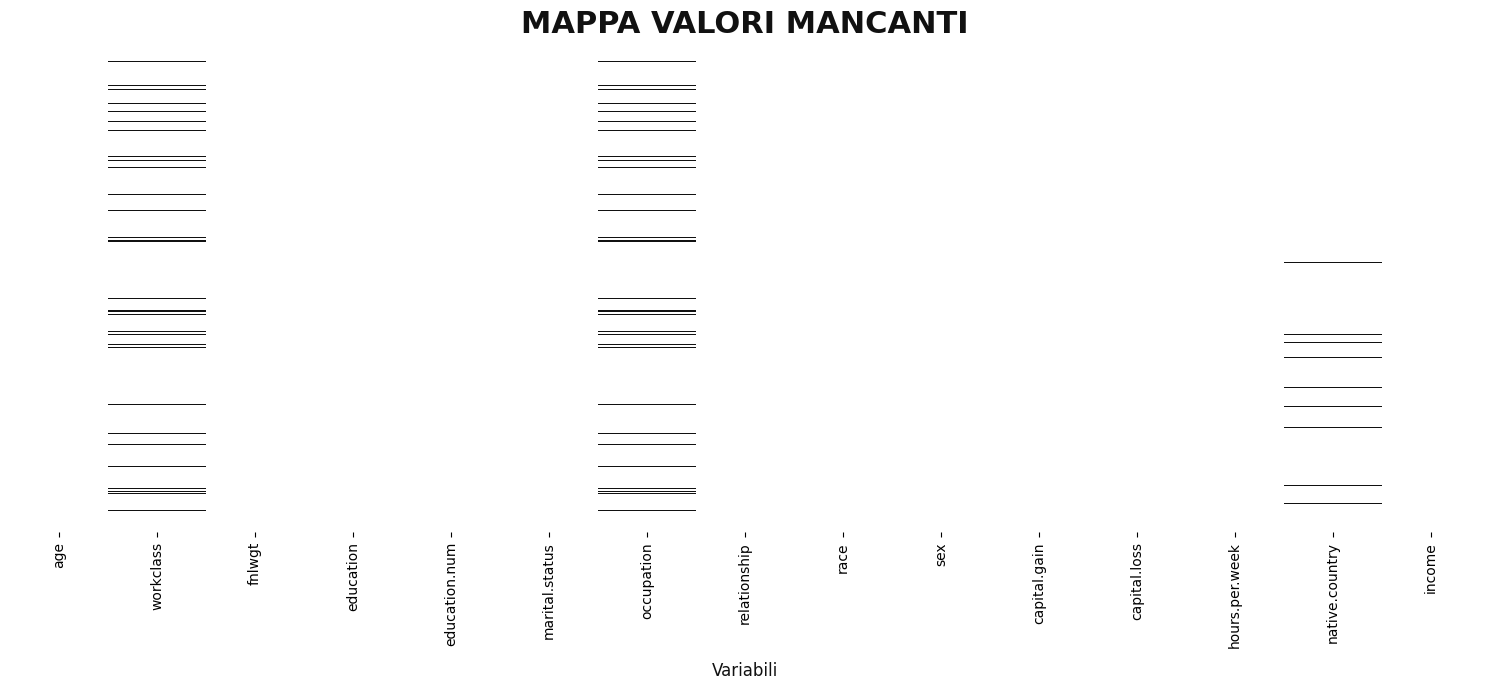
\includegraphics[width=\linewidth]{figures/mappa_valori_mancanti_2.png}
    \caption{\textbf{Heatmap della co-occorrenza dei valori mancanti.} La sovrapposizione visiva tra \texttt{workclass} e \texttt{occupation} suggerisce un pattern strutturale: individui privi di informazione su una variabile tendono a presentare un valore mancante anche nella seconda.}
    \label{fig:missing_heatmap}
\end{figure}

\noindent
Analisi quantitativa della co-occorrenza:
\begin{itemize}
    \item \textbf{Entrambi mancanti (workclass E occupation):} 1.836 osservazioni (di cui 27 estese anche a \texttt{native.country})
    \item \textbf{Solo occupation mancante:} 7 osservazioni
    \item \textbf{Solo native.country mancante:} 556 osservazioni
    \item \textbf{Dati completi:} 30.162 osservazioni (92.63\%)
\end{itemize}

\noindent
La concentrazione della mancanza congiunta (quasi il 100\% della mancanza in \texttt{workclass} si riflette in \texttt{occupation}) suggerisce un meccanismo \textit{Missing Not At Random} (MNAR), legato probabilmente a soggetti non occupati o categorie non censite, piuttosto che a un errore casuale di inserimento.

\subsubsection{Strategia di trattamento adottata}

Considerato che:
\begin{enumerate}
    \item La mancanza è strutturata e non casuale (MNAR)
    \item L'imputazione di variabili categoriche così specifiche potrebbe introdurre bias significativi nel modello predittivo
    \item Le variabili interessate sono solo 3 su 15, e la perdita totale è contenuta al \textbf{7.44\%}
    \item Il dataset rimane statisticamente robusto anche dopo la rimozione, conservando \textbf{30.139} osservazioni valide
\end{enumerate}

\noindent
Si è optato per la \textbf{listwise deletion}. Questa scelta garantisce la massima qualità del dato per le fasi successive di training, a fronte di una riduzione del campione considerata accettabile.

\begin{figure}[H]
    \centering
    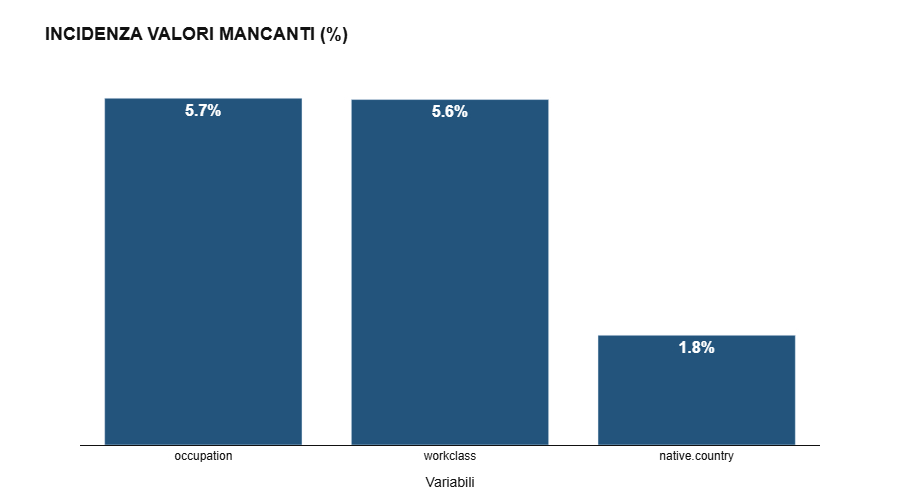
\includegraphics[width=\linewidth]{figures/incidenza_valori_mancanti.png}
    \caption{\textbf{Distribuzione percentuale dei valori mancanti per variabile.} Le variabili \texttt{occupation} (5.66\%), \texttt{workclass} (5.64\%) e \texttt{native.country} (1.79\%) rappresentano l'interezza dei dati mancanti nel dataset originale di 32.561 record.}
    \label{fig:missing_bar}
\end{figure}
\subsection{Analisi Descrittiva delle Variabili Categoriche}

\subsubsection{Strategia di analisi}

Per ciascuna variabile categorica è stata condotta un'analisi bidimensionale secondo il seguente protocollo:
\begin{enumerate}
    \item \textbf{Distribuzione marginale (assoluta e relativa):} frequenze e grafici a barre per visualizzare la cardinalità e il bilanciamento interno di ogni feature
    \item \textbf{Distribuzione condizionata rispetto al target:} suddivisione delle frequenze per classe di reddito, visualizzazione mediante barre affiancate o stacked
    \item \textbf{Proporzione della classe positiva per categoria:} calcolo della probabilità $P(income = >50K | \text{categoria})$ al fine di identificare categorie fortemente associate al reddito alto
\end{enumerate}

\noindent
Tale approccio consente di valutare sia la frequenza assoluta delle categorie (relevance per problemi di rarità) che la loro capacità discriminante, rilevante per la modellazione.

\subsubsection{Analisi di \texttt{workclass}}

\begin{figure}[H]
    \centering
    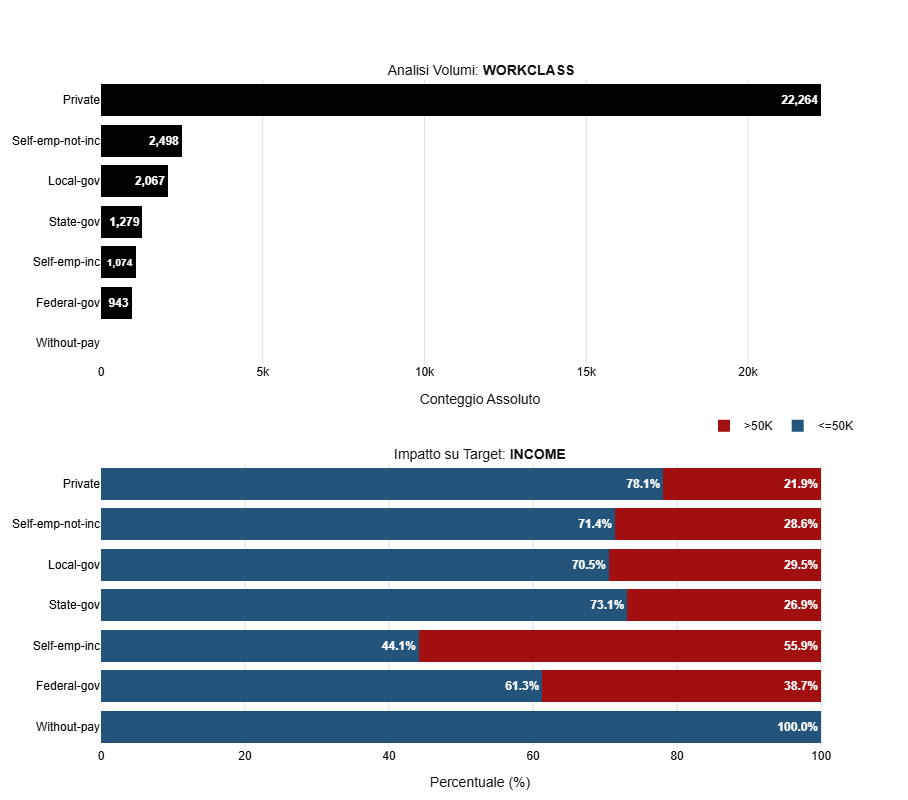
\includegraphics[width=0.9\linewidth]{figures/workclass1.png}
    \caption{\textbf{Analisi bivariata \texttt{workclass} vs \texttt{income}.} In alto: distribuzione assoluta delle categorie di classe lavorativa. In basso: proporzione della classe positiva per categoria, mostrando la capacità discriminante.}
    \label{fig:eda_workclass}
\end{figure}

\noindent
Osservazioni principali:
\begin{itemize}
    \item \textbf{Cardinalità:} 8 categorie, dominata da \textit{Private}
    \item \textbf{Discriminanza:} \textit{Self-emp-inc} (lavoratori autonomi incorporati) registra la probabilità più elevata di reddito $>50K$ (55.7\%), suggerendo una forte capacità predittiva
    \item \textbf{Categorie rare:} \textit{Without-pay e Never-worked} sono outlier, rappresentando categorie patologiche
\end{itemize}

\subsubsection{Analisi di \texttt{education}}

\begin{figure}[H]
    \centering
    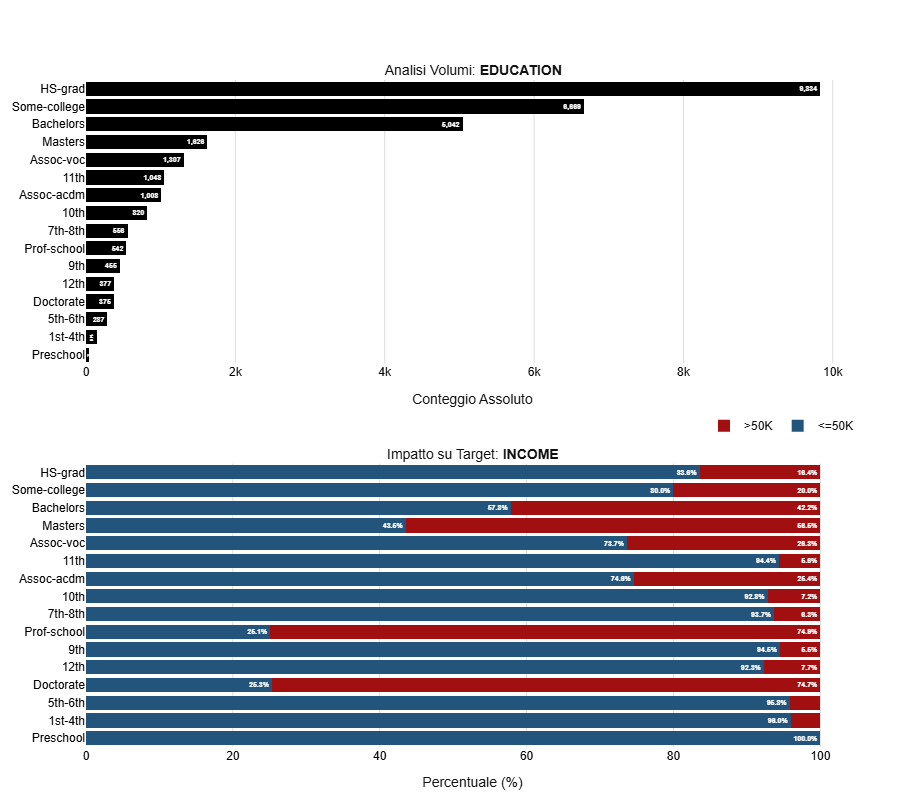
\includegraphics[width=\linewidth]{figures/education1.png}
    \caption{\textbf{Analisi bivariata \texttt{education} vs \texttt{income}.} La distribuzione mostra un ordinamento naturale (da Preschool a Doctorate).}
    \label{fig:eda_education}
\end{figure}

\noindent
Osservazioni principali:
\begin{itemize}
    \item \textbf{Ordinamento naturale:} A differenza di altre categoriche, education segue un ordinamento intrinseco (da meno a più istruzione)
    \item \textbf{Monotonicità della proporzione:} La probabilità $P(income = >50K)$ cresce in modo quasi monotono al crescere della scolarità: 0\% per Preschool, 74\% per Doctorate
    \item \textbf{Cardinalità:} 16 categorie, potenzialmente alta per alberi non ottimizzati
    \item \textbf{Alternativa numerica:} Esiste una variabile \texttt{education.num} che codifica numericamente questo ordinamento, suggerendo ridondanza informativa (da valutare in feature selection)
\end{itemize}

\subsubsection{Analisi di \texttt{marital.status}}

\begin{figure}[H]
    \centering
    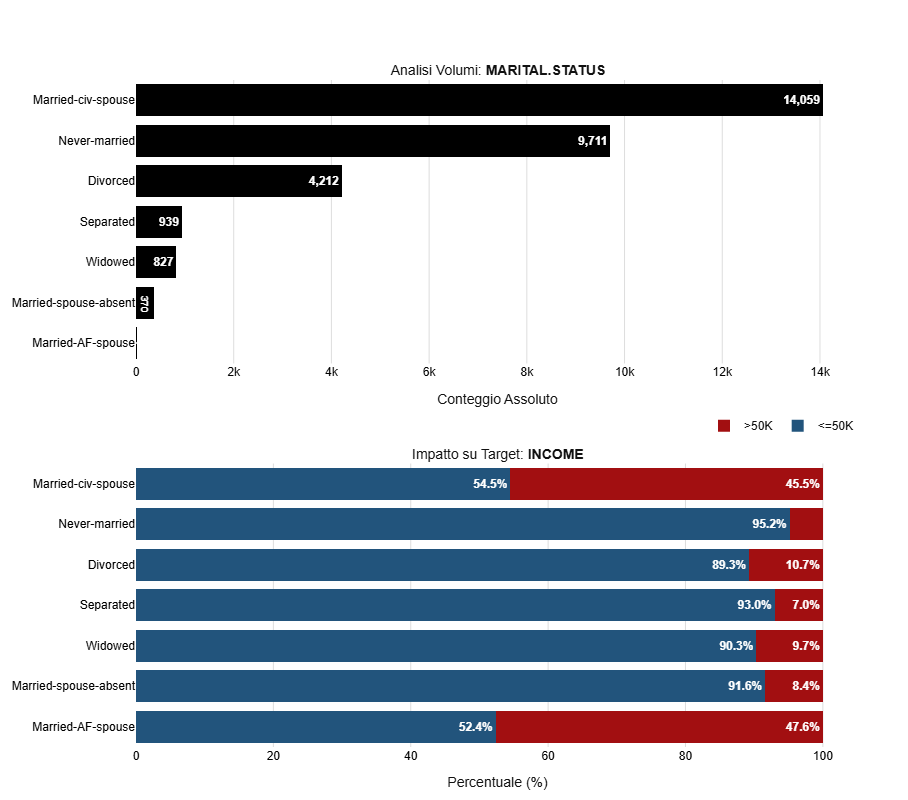
\includegraphics[width=0.9\linewidth]{figures/maritalstatus1.png}
    \caption{\textbf{Analisi bivariata \texttt{marital.status} vs \texttt{income}.} Lo stato civile emerge come uno dei predittori categorici più forti. Aver cessato il rapporto con il partner o non averne mai avuto mostra la bassa potenzialità a redditi $>50K$.}
    \label{fig:eda_marital}
\end{figure}

\noindent
Osservazioni principali:
\begin{itemize}
    \item \textbf{Discriminanza elevata:} Le categorie \textit{Married-civ-spouse} (44.7\%) e \textit{Married-AF-spouse} (43.5\%) mostrano probabilità di reddito alto quasi doppia rispetto alla media
    \item \textbf{Implicazione demografica:} Il matrimonio è storicamente associato a stabilità lavorativa e reddito più elevato, coerente con i dati
    \item \textbf{Sbilanciamento interno:} \textit{Never-married} è la seconda categoria più numerosa ma con la probabilità di reddito alto più bassa (4.6\%)
    \item \textbf{Cardinalità:} 7 categorie, gestibile
\end{itemize}

\subsubsection{Analisi di \texttt{occupation}}

\begin{figure}[H]
    \centering
    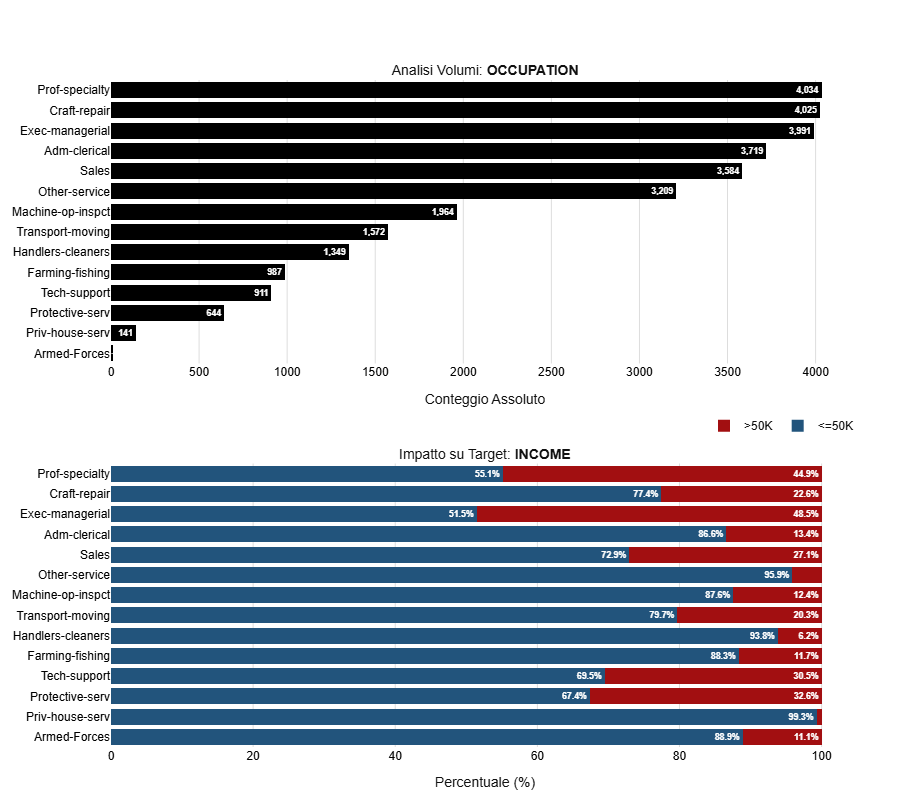
\includegraphics[width=\linewidth]{figures/occupation1.png}
    \caption{\textbf{Analisi bivariata \texttt{occupation} vs \texttt{income}.} Le professioni manageriali e specialistiche registrano le proporzioni più elevate di reddito alto.}
    \label{fig:eda_occupation}
\end{figure}

\noindent
Osservazioni principali:
\begin{itemize}
    \item \textbf{Discriminanza per ruolo:} \textit{Exec-managerial} (48.4\%) e \textit{Prof-specialty} (44.9\%) emergono come categorie ad alta capacità predittiva
    \item \textbf{Bimodalità implicita:} Le professioni si scindono chiaramente in "alte" (reddito > 50K probabile) e "basse" (es. \textit{Other-service} 4.2\%)
    \item \textbf{Cardinalità:} 14 categorie, ragionevolmente alta ma contenuta
\end{itemize}

\subsubsection{Analisi di \texttt{relationship}}

\begin{figure}[H]
    \centering
    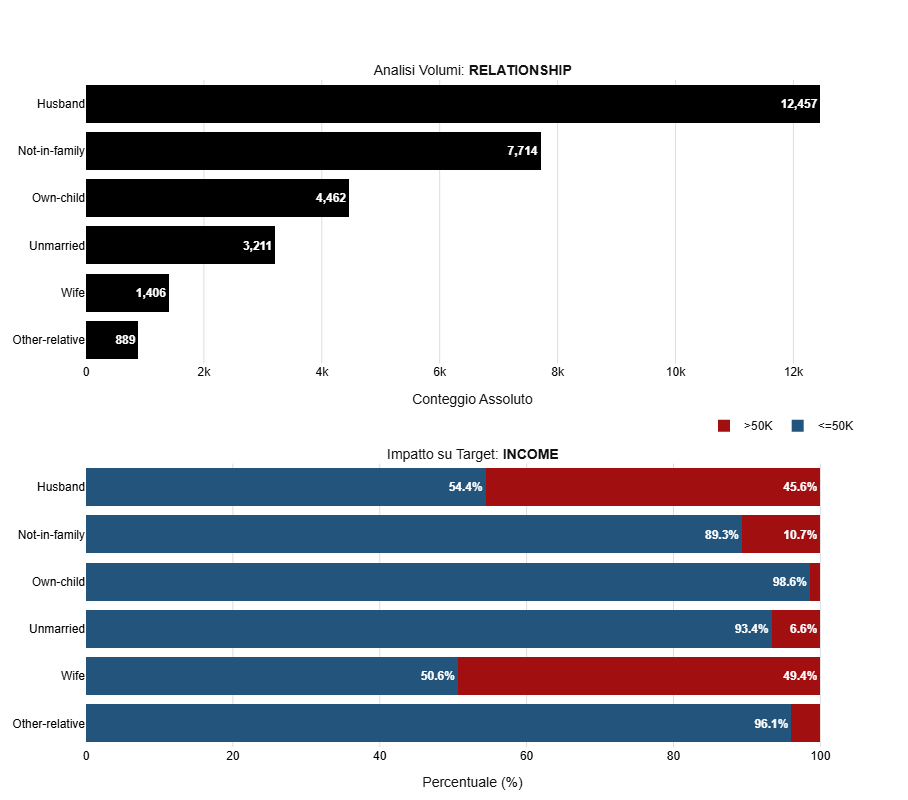
\includegraphics[width=\linewidth]{figures/relationship1.png}
    \caption{\textbf{Analisi bivariata \texttt{relationship} vs \texttt{income}.} Il ruolo familiare è strettamente correlato al target, con \textit{Husband} e \textit{Wife} dominanti nella classe positiva.}
    \label{fig:eda_relationship}
\end{figure}

\noindent
Osservazioni principali:
\begin{itemize}
    \item \textbf{Sovrapposizione con marital.status:} Esiste una forte relazione naturale con marital.status
    \item \textbf{Cardinalità bassa:} 6 categorie
\end{itemize}

\subsubsection{Analisi di \texttt{race}}

\begin{figure}[H]
    \centering
    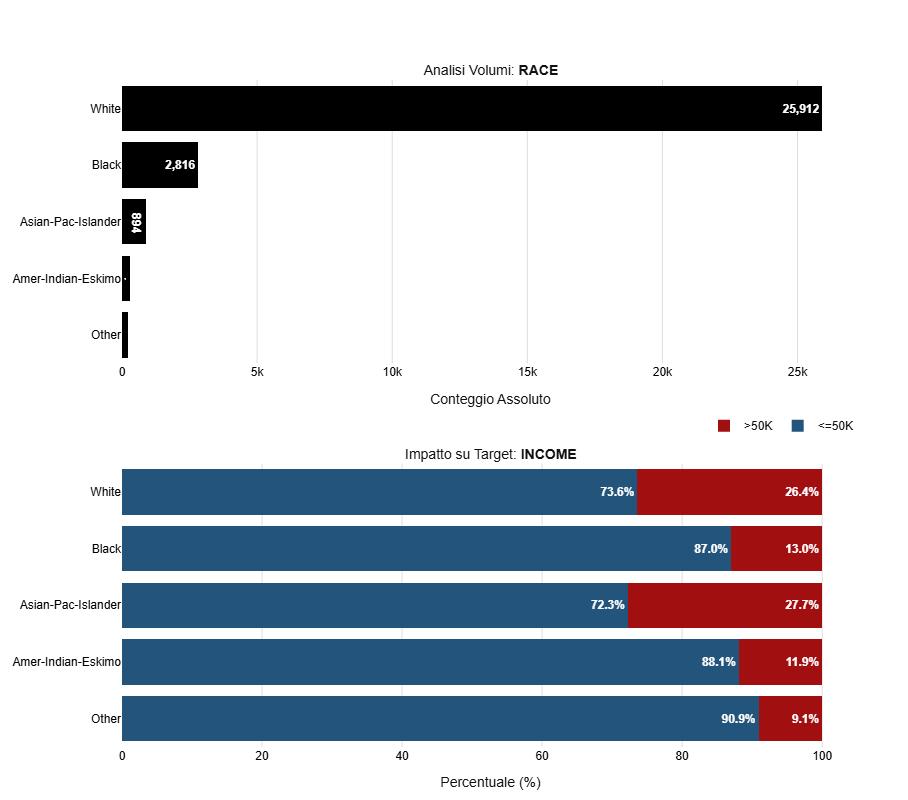
\includegraphics[width=0.9\linewidth]{figures/race1.png}
    \caption{\textbf{Analisi bivariata \texttt{race} vs \texttt{income}.} Emerge un marcato sbilanciamento campionario (> 86\% White) e disparità nelle proporzioni di reddito per gruppo etnico.}
    \label{fig:eda_race}
\end{figure}

\noindent
Osservazioni principali:
\begin{itemize}
    \item \textbf{Sbilanciamento campionario estremo:} White rappresenta il 86\% della popolazione, Asian-Pac-Islander circa il 3.0\%, altre categorie < 1 \%
    \item \textbf{Disparità reddituali:} Asian-Pac-Islander registra la proporzione più elevata di reddito alto (27.7\%), seguita da White (26.4\%)
    \item \textbf{Sensibilità etica:} La variabile race in contesti predittivi sensibili richiede cautela nell'interpretazione e nella comunicazione dei risultati
\end{itemize}

\subsubsection{Analisi di \texttt{sex}}

\begin{figure}[H]
    \centering
    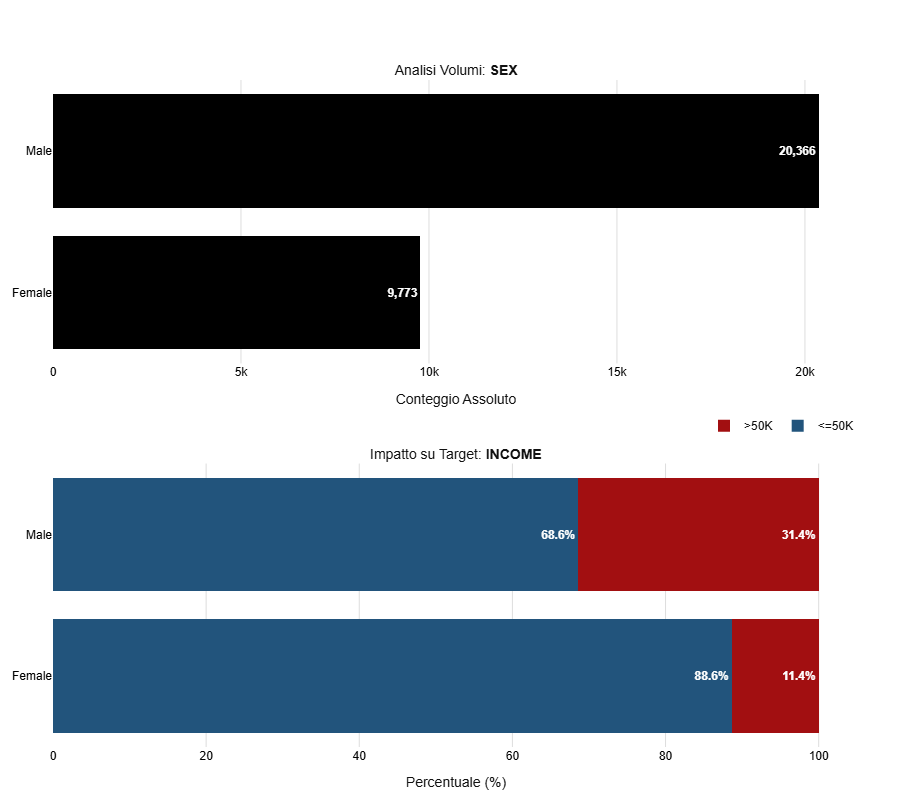
\includegraphics[width=\linewidth]{figures/sex1.png}
    \caption{\textbf{Analisi bivariata \texttt{sex} vs \texttt{income}.} Gap di genere marcato: il 31.4\% degli uomini ma solo 11.4\% delle donne raggiunge reddito > 50K nel dataset.}
    \label{fig:eda_sex}
\end{figure}

\noindent
Osservazioni principali:
\begin{itemize}
    \item \textbf{Gap reddituario:} Differenza proporzionale di 20 punti percentuali (31.4\% vs 11.4\%)
    \item \textbf{Cardinalità minima:} 2 categorie (possibilità di conversione binaria diretta per alcuni algoritmi)
    \item \textbf{Implicazione sociologica:} Il gap riflette disparità storiche nel mercato del lavoro, preservate nel dataset censuario
\end{itemize}

\subsubsection{Analisi di \texttt{native.country}}

\begin{figure}[H]
    \centering
    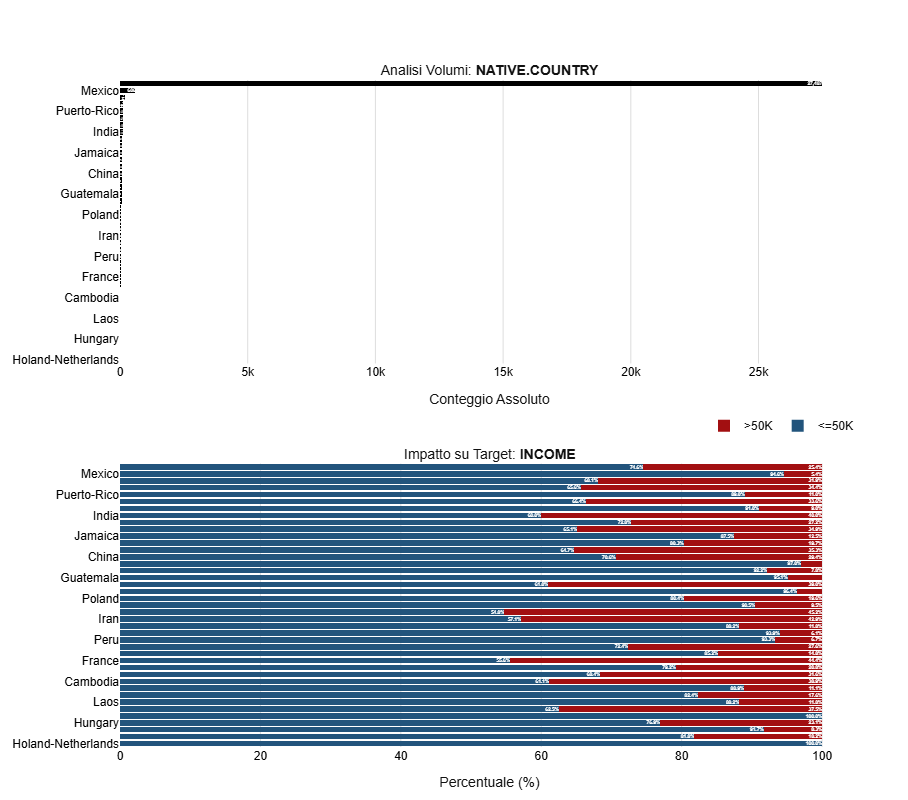
\includegraphics[width=\linewidth]{figures/nativecountry1.png}
    \caption{\textbf{Analisi bivariata \texttt{native.country} vs \texttt{income}.} Si osserva un'estrema polarizzazione verso gli \textit{United-States} (91.2\%), con una dispersione di micro-categorie per le restanti 40 nazioni.}
    \label{fig:eda_country}
\end{figure}

\noindent
Osservazioni principali:
\begin{itemize}
    \item \textbf{Dominanza statistica:} Gli \textit{United-States} rappresentano il \textbf{91.2\%} del campione (27.487 osservazioni) con un tasso di reddito elevato ($>50K$) del 25.4\%, valore che funge da baricentro per l'intero dataset.
    \item \textbf{Sparsità estrema:} Nonostante vi siano 41 valori unici, solo il \textbf{Mexico} (606 obs, 2.0\%) supera l'1\% di rappresentatività oltre agli USA. Paesi come \textit{Philippines} (0.6\%) e \textit{Germany} (0.4\%) mostrano frequenze troppo basse per garantire robustezza statistica individuale.
    \item \textbf{Eterogeneità del Target:} Si notano forti variazioni nel tasso di reddito tra le minoranze; ad esempio, \textit{Taiwan} (45.2\%) e \textit{Iran} (42.9\%) mostrano incidenze di reddito elevato molto superiori alla media, mentre \textit{Columbia} (3.6\%) e \textit{Dominican-Republic} (3.0\%) presentano valori minimi.
    \item \textbf{Implicazione di Feature Engineering:} L'alta cardinalità combinata con la presenza di categorie quasi nulle (es. \textit{Holand-Netherlands} con 1 sola osservazione) rende necessaria un'aggregazione in macro-aree geografiche o una binarizzazione ("USA" vs "Others") per prevenire l'overfitting e ridurre la dimensionalità dello spazio delle feature.
\end{itemize}


\subsection{Analisi Multivariata: Segmentazione per Genere}

Al fine di identificare potenziali bias demografici o differenze strutturali nella capacità discriminante delle \textit{feature}, è stata condotta un'analisi multivariata segmentando le variabili categoriche per la variabile \texttt{sex}. 

\begin{enumerate}[label=(\roman*)]
    \item \textbf{Obiettivo:} valutare come l'impatto delle singole variabili sul target vari tra uomini e donne, identificando categorie che potrebbero avere un peso predittivo differente nei due sottogruppi.
    \item \textbf{Metodologia visuale:} sono stati generati grafici a barre orizzontali normalizzati al 100\% (\textit{barnorm='percent'}). Questa scelta consente di confrontare direttamente le probabilità condizionate $P(income > 50K | feature, sex)$, eliminando l'effetto distorsivo dei volumi assoluti (essendo il campione maschile numericamente superiore).
\end{enumerate}

\begin{figure}[H]
    \centering
    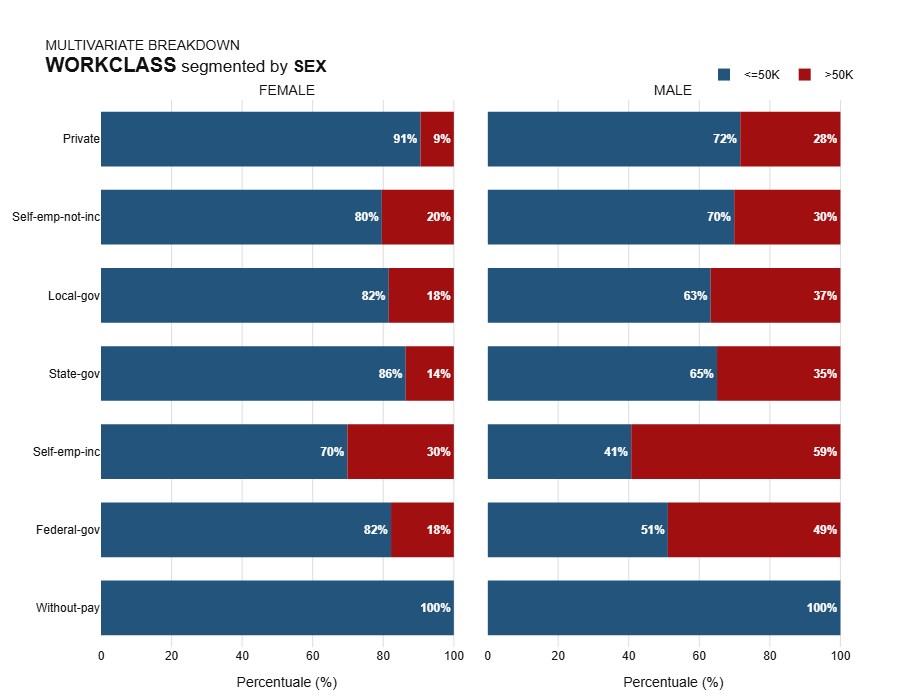
\includegraphics[width=\linewidth]{figures/worklass2.png} 
    \caption{\textbf{Analisi multivariata segmentata per sesso.} Il grafico mostra come il sesso femminile tende ad avere un reddito inferiore al 50K. Mentre solo in \texttt{self-emp-inc} gli uomini sono per il 59\% con redditi superiori a 50K.}
    \label{fig:worklass2.png}
\end{figure}

\begin{figure}[H]
    \centering
    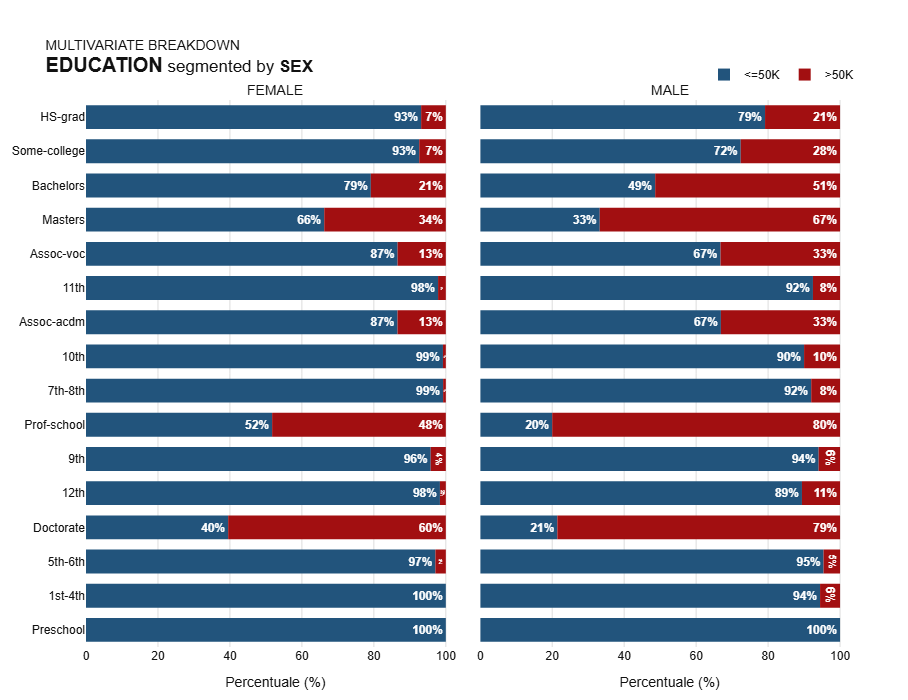
\includegraphics[width=\linewidth]{figures/education2.png} 
    \caption{\textbf{Analisi multivariata segmentata per sesso.} I generi mostrano che un alto livello di istruzione è associato a un reddito superiore, ma con differenze significative tra uomini e donne anche se seguono lo stesso andamento.}
    \label{fig:education2.png}
\end{figure}

\begin{figure}[H]
    \centering
    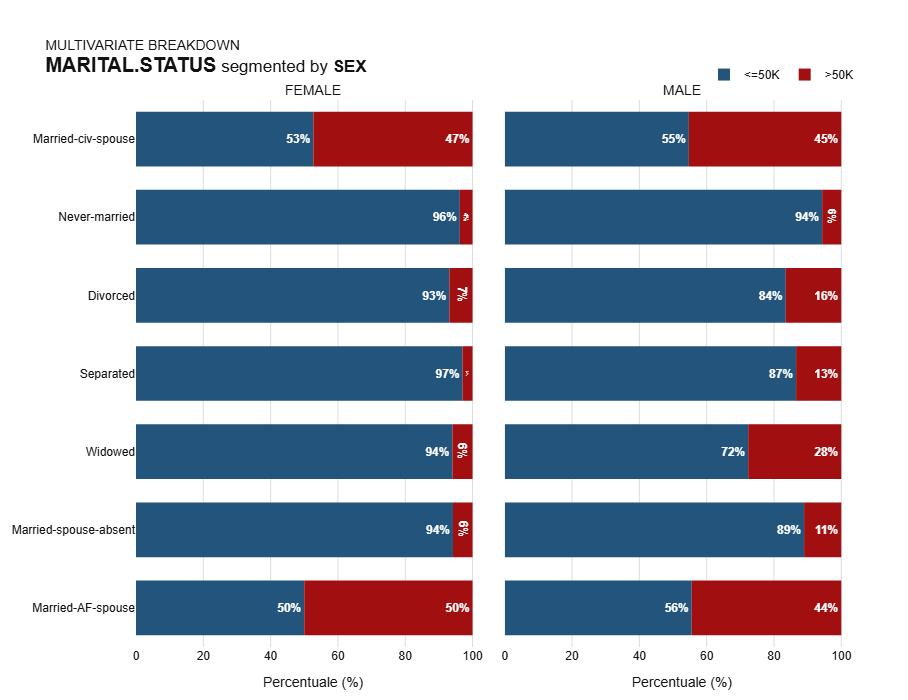
\includegraphics[width=\linewidth]{figures/maritalsstatus2.png} 
    \caption{\textbf{Analisi multivariata segmentata per sesso.} \texttt{marital-status} ci mostra che tra i generi nelle modalità "Married-civ-spouse" e "Married-AF-spouse" le donne hanno una percentuale di redditi superiori a 50K più bassa rispetto agli uomini. Per il resto gli uomini hanno sempre una percentuale più alta di redditi superiori a 50K.}
    \label{fig:aritalsstatus2.png}
\end{figure}

\begin{figure}[H]
    \centering
    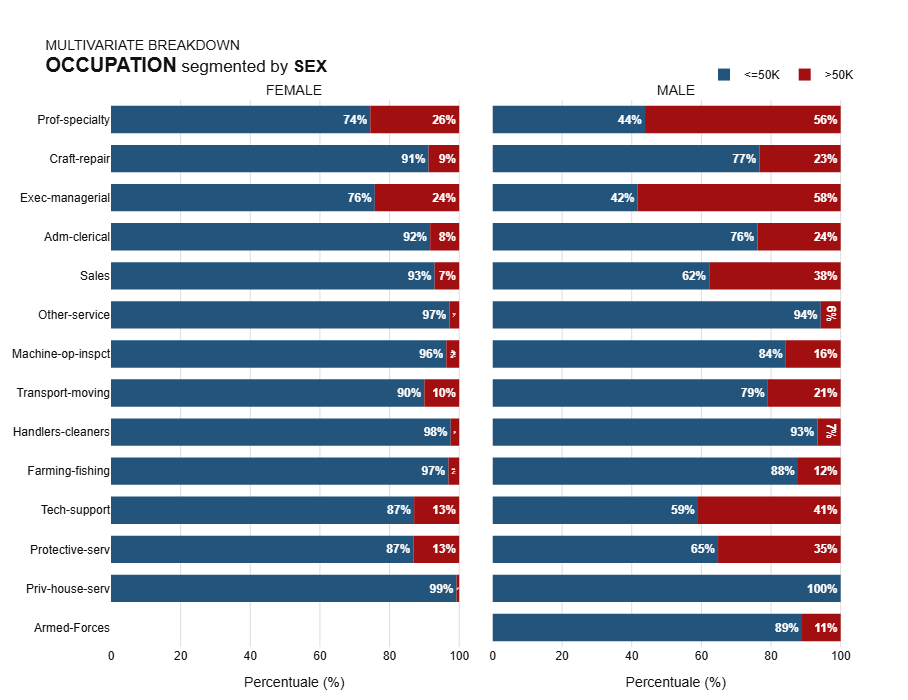
\includegraphics[width=\linewidth]{figures/occupation2.png} 
    \caption{\textbf{Analisi multivariata segmentata per sesso.} L'occupazione non è immune al gap di genere: in quasi tutte le categorie, gli uomini mostrano una proporzione più elevata di redditi > 50K rispetto alle donne.}
    \label{fig:occupation2.png}
\end{figure}

\begin{figure}[H]
    \centering
    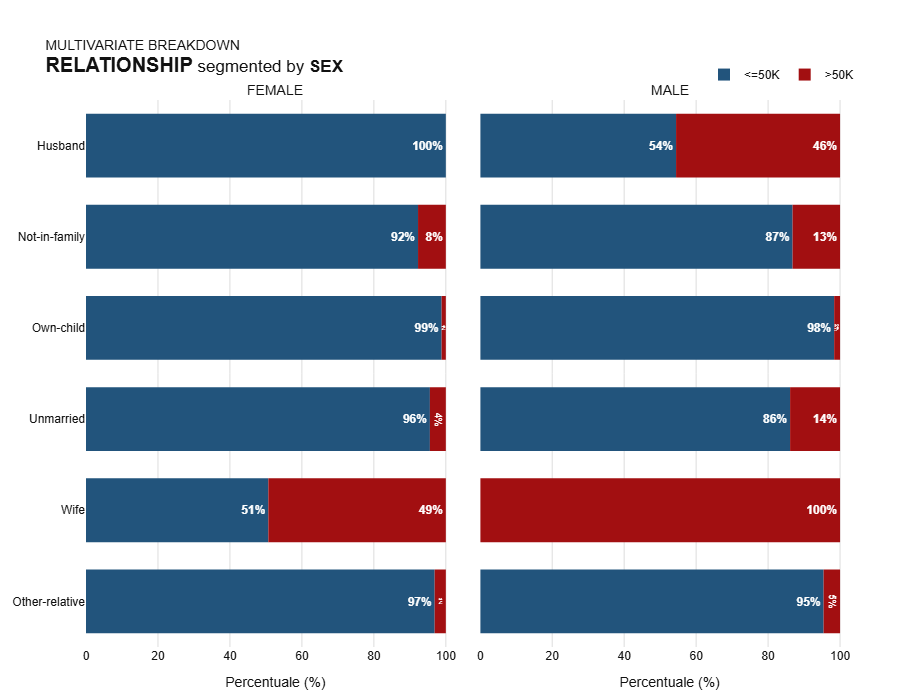
\includegraphics[width=\linewidth]{figures/relationship2.png} 
    \caption{\textbf{Analisi multivariata segmentata per sesso.} Il ruolo familiare mostra un pattern simile a marital.status, con gli uomini che tendono ad avere una maggiore proporzione di redditi elevati in quasi tutte le categorie, evidenziando un possibile effetto di interazione tra ruolo familiare e genere. Si evidenzia che le donne che sono "Wife" hanno una percentuale di redditi superiori a 50K più bassa rispetto agli uomini che sono "Husband".}
    \label{fig:relationship2.png}
\end{figure}

\begin{figure}[H]
    \centering
    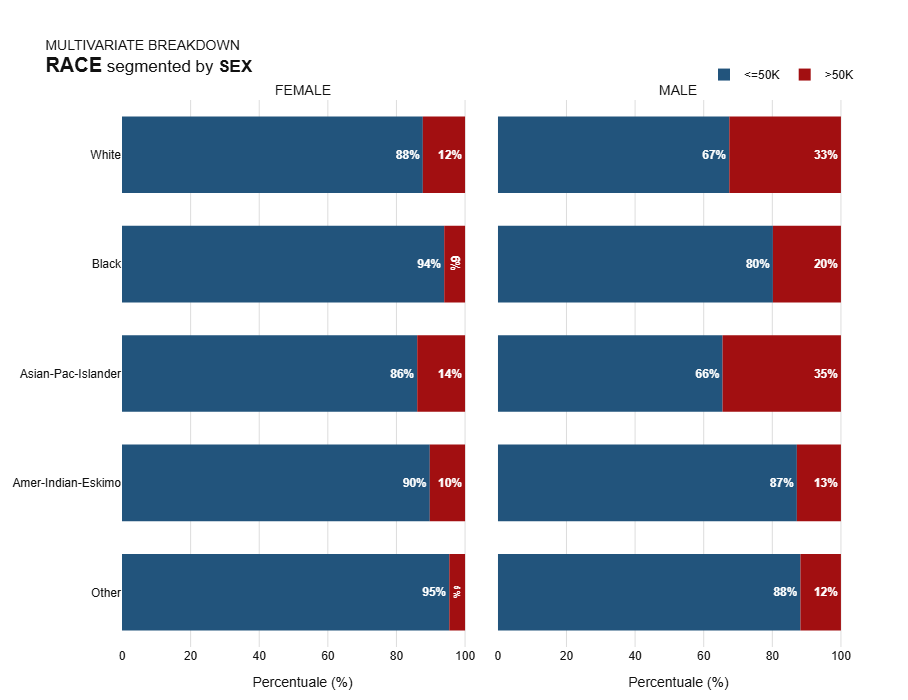
\includegraphics[width=\linewidth]{figures/race2.png} 
    \caption{\textbf{Analisi multivariata segmentata per sesso.} L'etnia mostra differenze di reddito tra i generi, con gli uomini che tendono ad avere una maggiore proporzione di redditi elevati rispetto alle donne in tutte le categorie etniche.}
    \label{fig:race2.png}
\end{figure}

\begin{figure}[H]
    \centering
    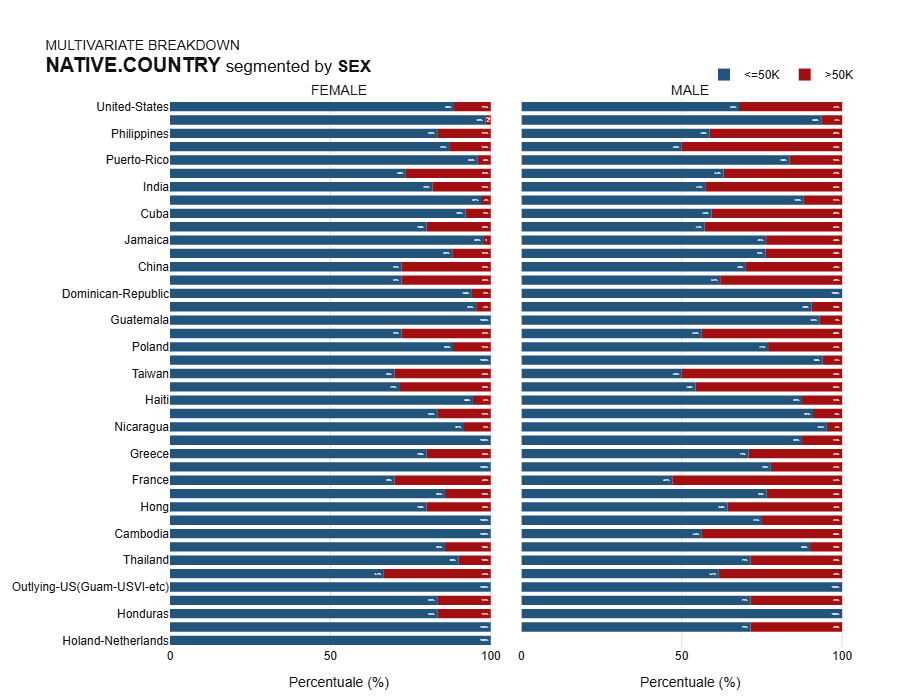
\includegraphics[width=\linewidth]{figures/nativecountry2.png} 
    \caption{\textbf{Analisi multivariata segmentata per sesso.} La nazionalità mostra un pattern di reddito più elevato per gli uomini rispetto alle donne in quasi tutte le categorie, con alcune eccezioni.}
    \label{fig:nativecountry2.png}
\end{figure}

\newpage

\subsection{Analisi Descrittiva delle Variabili Numeriche}

\subsubsection{Protocollo di analisi univariata}

Per ogni feature continua è stata condotta un'analisi distributzionale secondo:
\begin{enumerate}
    \item \textbf{Istogramma con kernel density estimate (KDE):} Visualizzazione della forma distributiva
    \item \textbf{Box plot:} Identificazione di outlier mediante IQR (intervallo interquartile)
    \item \textbf{Statistiche descrittive complete:} Media, mediana, std, min, max, quantili 25/75, Skewness, Kurtosis
    \item \textbf{Confronto condizionato sul target:} Overlay di distribuzioni per reddito $\leq 50K$ vs $> 50K$
\end{enumerate}

\noindent
Le metriche di forma distributiva sono critiche per valutare la necessità di trasformazioni (es. Box-Cox, log-transform) prima della modellazione con algoritmi sensibili alle code pesanti (es. regressione lineare, SVM).
% --- TABELLA RIEPILOGATIVA GENERALE ---
\subsubsection{Quadro Statistico Globale}

\begin{table}[H]
    \centering
    \caption{Statistiche descrittive globali delle variabili numeriche (N = 30.139)}
    \begin{adjustbox}{width=\textwidth,center}
    \begin{tabular}{lrrrrrrrrrrr}
        \toprule
        \textbf{Variabile} & \textbf{Media} & \textbf{Mediana} & \textbf{Moda} & \textbf{Dev. Std} & \textbf{CV} & \textbf{IQR} & \textbf{Min} & \textbf{Max} & \textbf{Skew} & \textbf{Kurt} \\
        \midrule
        age & 38.44 & 37.00 & 36.00 & 13.13 & 0.34 & 19.00 & 17.00 & 90.00 & 0.53 & -0.15 \\
        fnlwgt & 189,795 & 178,417 & 203,488 & 105,658 & 0.56 & 119,977 & 13,769 & 1,484,705 & 1.46 & 6.40 \\
        education.num & 10.12 & 10.00 & 9.00 & 2.55 & 0.25 & 4.00 & 1.00 & 16.00 & -0.30 & 0.64 \\
        capital.gain & 1,092.84 & 0.00 & 0.00 & 7,409.11 & 6.78 & 0.00 & 0.00 & 99,999 & 11.90 & 153.55 \\
        capital.loss & 88.44 & 0.00 & 0.00 & 404.45 & 4.57 & 0.00 & 0.00 & 4,356 & 4.52 & 19.49 \\
        hours.per.week & 40.93 & 40.00 & 40.00 & 11.98 & 0.29 & 5.00 & 1.00 & 99.00 & 0.33 & 3.17 \\
        \bottomrule
    \end{tabular}
    \end{adjustbox}
\end{table}

\vspace{1cm}

\newpage
% --- ANALISI DETTAGLIATA AGE ---
\subsubsection{Analisi di \texttt{age}}

\begin{table}[H]
    \centering
    \footnotesize
    \caption{Dettaglio \texttt{age} per gruppo di reddito e analisi del Delta}
    
    \textbf{Tabella A: Statistiche per Gruppo} \\
    \begin{tabular}{lrrrrrrrr}
        \toprule
        \textbf{income} & \textbf{Conteggio} & \textbf{Media} & \textbf{Mediana} & \textbf{Dev. Std} & \textbf{Min} & \textbf{Max} & \textbf{IQR} & \textbf{Skew} \\
        \midrule
        $\leq 50K$ & 22,633.00 & 36.61 & 34.00 & 13.46 & 17.00 & 90.00 & 19.00 & 0.74 \\
        $> 50K$ & 7,506.00 & 43.96 & 43.00 & 10.27 & 19.00 & 90.00 & 15.00 & 0.46 \\
        \bottomrule
    \end{tabular}

    \vspace{0.4cm}
    
    \textbf{Tabella B: Delta Report ($>50K$ vs $\leq 50K$)} \\
    \begin{tabular}{clrrrr}
        \toprule
        \textbf{ID} & \textbf{Metrica} & \textbf{$\leq 50K$ (Base)} & \textbf{$> 50K$ (Confronto)} & \textbf{Diff. Assoluta} & \textbf{Diff. \%} \\
        \midrule
        0 & Media & 36.61 & 43.96 & +7.35 & +20.07\% \\
        1 & Mediana & 34.00 & 43.00 & +9.00 & +26.47\% \\
        2 & Dev. Std & 13.46 & 10.27 & -3.19 & -23.70\% \\
        3 & IQR & 19.00 & 15.00 & -4.00 & -21.05\% \\
        \bottomrule
    \end{tabular}
\end{table}

\begin{figure}[H]
    \centering
    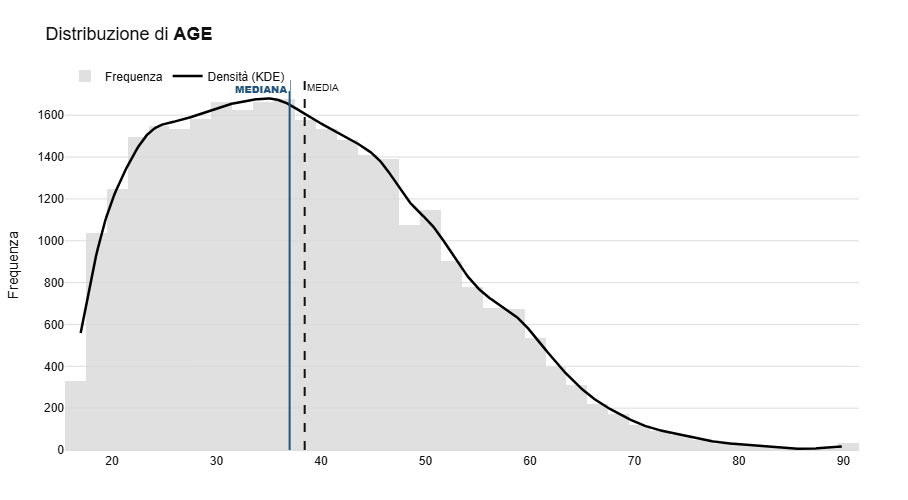
\includegraphics[width=1\linewidth]{figures/age1.png} % Sostituisci con il nome del tuo file immagine
    \caption{\textbf{Distribuzione di Age.} La discrepanza tra media e mediana evidenzia l'asimmetria positiva della distribuzione demografica.}
    \label{fig:uni_age}
\end{figure}

\begin{figure}[H]
    \centering
    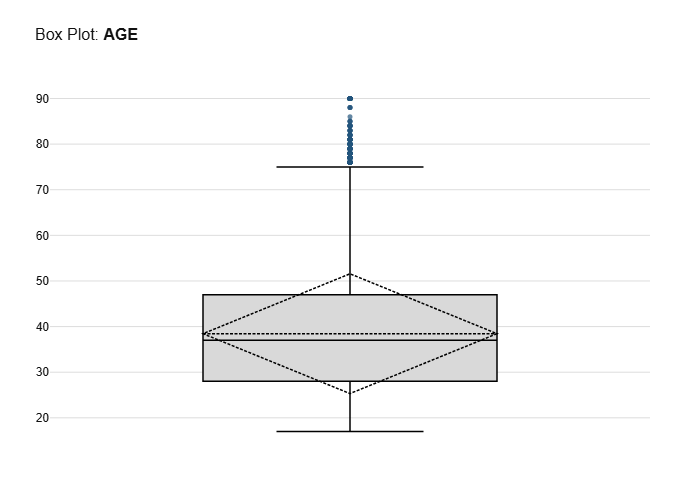
\includegraphics[width=0.8\linewidth]{figures/age_b.png} % Sostituisci con il nome del tuo file immagine
    \caption{\textbf{Boxplot di Age.} il 50\% dei valori si trova tra 30 e 50 anni.}
    \label{fig:age_b.png}
\end{figure}

\noindent
\textbf{Interpretazione:}
\begin{itemize}
    \item La distribuzione rimane approssimativamente normale con una leggera coda destra, tipica delle popolazioni lavorative.
    \item \textbf{Differenza bivariata su target:} Il delta tra le classi di reddito rimane significativo, suggerendo che l'anzianità favorisca redditi elevati fino alla soglia del pensionamento.
\end{itemize}

\newpage
% --- ANALISI DETTAGLIATA FNLWGT ---
\subsubsection{Analisi di \texttt{fnlwgt} (Final Weight)}

\begin{table}[H]
    \centering
    \footnotesize
    \caption{Dettaglio \texttt{fnlwgt} per gruppo di reddito e analisi del Delta}
    
    \textbf{Tabella A: Statistiche per Gruppo} \\
    \begin{tabular}{lrrrrrrrr}
        \toprule
        \textbf{income} & \textbf{Conteggio} & \textbf{Media} & \textbf{Mediana} & \textbf{Dev. Std} & \textbf{Min} & \textbf{Max} & \textbf{IQR} & \textbf{Skew} \\
        \midrule
        $\leq 50K$ & 22,633.00 & 190,342.15 & 179,508.00 & 106,575.12 & 13,769.00 & 1,484,705.00 & 122,097.00 & 1.48 \\
        $> 50K$ & 7,506.00 & 188,145.28 & 176,171.00 & 102,835.03 & 14,878.00 & 1,226,583.00 & 111,992.50 & 1.41 \\
        \bottomrule
    \end{tabular}

    \vspace{0.4cm}
    
    \textbf{Tabella B: Delta Report ($>50K$ vs $\leq 50K$)} \\
    \begin{tabular}{clrrrr}
        \toprule
        \textbf{ID} & \textbf{Metrica} & \textbf{$\leq 50K$ (Base)} & \textbf{$> 50K$ (Confronto)} & \textbf{Diff. Assoluta} & \textbf{Diff. \%} \\
        \midrule
        0 & Media & 190,342.15 & 188,145.28 & -2,196.87 & -1.15\% \\
        1 & Mediana & 179,508.00 & 176,171.00 & -3,337.00 & -1.86\% \\
        2 & Dev. Std & 106,575.12 & 102,835.03 & -3,740.08 & -3.51\% \\
        3 & IQR & 122,097.00 & 111,992.50 & -10,104.50 & -8.28\% \\
        \bottomrule
    \end{tabular}
\end{table}

\begin{figure}[H]
    \centering
    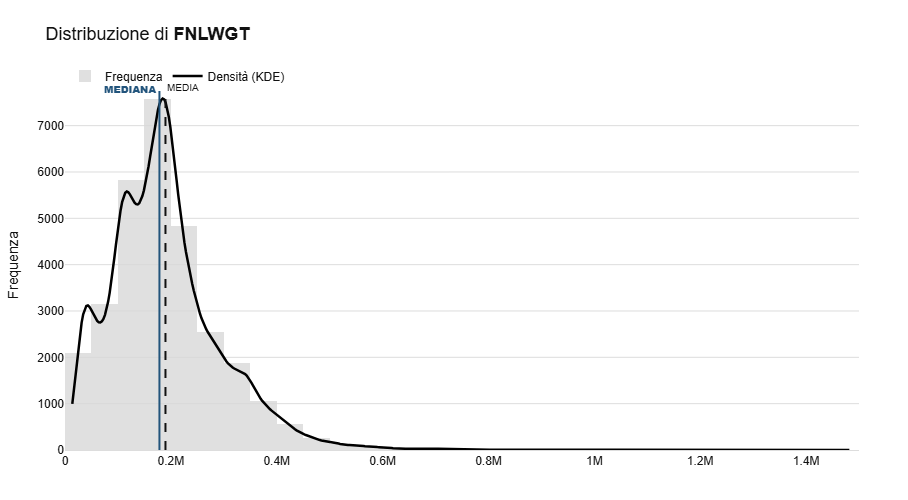
\includegraphics[width=1\linewidth]{figures/fnlwgt1.png}
    \caption{\textbf{Distribuzione di Final Weight.} La sovrapposizione quasi totale delle distribuzioni conferma l'assenza di potere predittivo.}
    \label{fig:uni_fnlwgt}
\end{figure}

\begin{figure}[H]
    \centering
    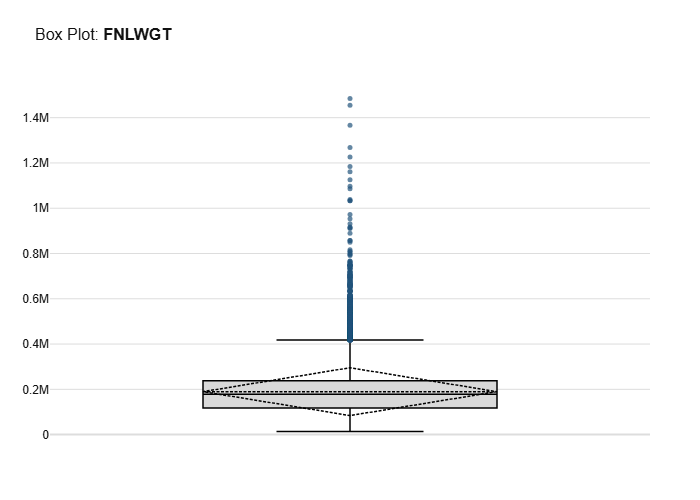
\includegraphics[width=0.8\linewidth]{figures/fnlwgt_b.png}
    \caption{\textbf{Boxplot di Final Weight.} valori estremi e outlier evidenti, con un range interquartile molto stretto.}
    \label{fig:fnlwgt_b.png}
\end{figure}

\noindent
\textbf{Interpretazione:}
\begin{itemize}
    \item La variabile mostra la sua natura di peso statistico amministrativo.
    \item L'alta kurtosis (+6.40) evidenzia la presenza di outlier estremi nella ponderazione demografica.
    \item \textbf{Decisione:} Si considera l'eventuale esclusione nelle fasi di addestramento dei modelli.
\end{itemize}

\newpage
% --- ANALISI DETTAGLIATA EDUCATION.NUM ---
\subsubsection{Analisi di \texttt{education.num}}

\begin{table}[H]
    \centering
    \footnotesize
    \caption{Dettaglio \texttt{education.num} per gruppo di reddito e analisi del Delta}
    
    \textbf{Tabella A: Statistiche per Gruppo} \\
    \begin{tabular}{lrrrrrrrr}
        \toprule
        \textbf{income} & \textbf{Conteggio} & \textbf{Media} & \textbf{Mediana} & \textbf{Dev. Std} & \textbf{Min} & \textbf{Max} & \textbf{IQR} & \textbf{Skew} \\
        \midrule
        $\leq 50K$ & 22,633.00 & 9.63 & 9.00 & 2.41 & 1.00 & 16.00 & 1.00 & -0.43 \\
        $> 50K$ & 7,506.00 & 11.61 & 12.00 & 2.37 & 2.00 & 16.00 & 3.00 & -0.30 \\
        \bottomrule
    \end{tabular}

    \vspace{0.4cm}
    
    \textbf{Tabella B: Delta Report ($>50K$ vs $\leq 50K$)} \\
    \begin{tabular}{clrrrr}
        \toprule
        \textbf{ID} & \textbf{Metrica} & \textbf{$\leq 50K$ (Base)} & \textbf{$> 50K$ (Confronto)} & \textbf{Diff. Assoluta} & \textbf{Diff. \%} \\
        \midrule
        0 & Media & 9.63 & 11.61 & +1.98 & +20.53\% \\
        1 & Mediana & 9.00 & 12.00 & +3.00 & +33.33\% \\
        2 & Dev. Std & 2.41 & 2.37 & -0.04 & -1.80\% \\
        3 & IQR & 1.00 & 3.00 & +2.00 & +200.00\% \\
        \bottomrule
    \end{tabular}
\end{table}

\begin{figure}[H]
    \centering
    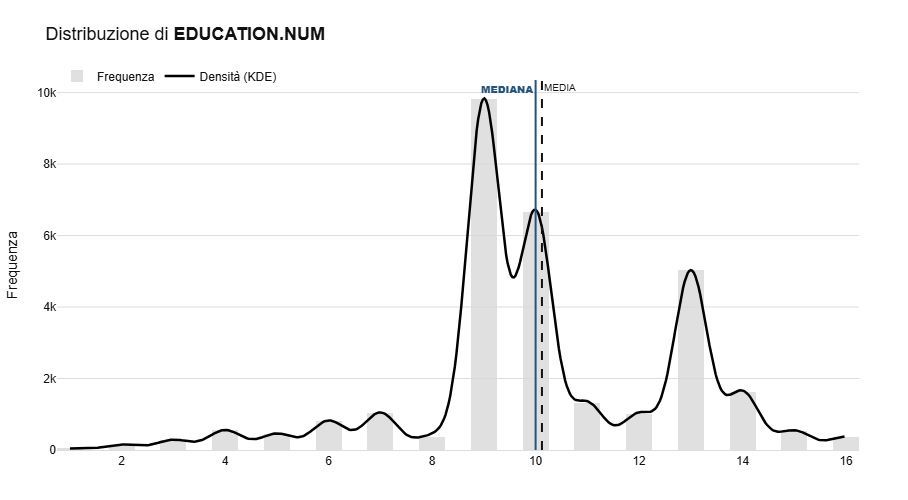
\includegraphics[width=1\linewidth]{figures/educationnum1.png}
    \caption{\textbf{Distribuzione di Education Num.} I picchi multipli riflettono la struttura a gradini dei cicli scolastici.}
    \label{fig:uni_edu}
\end{figure}

\begin{figure}[H]
    \centering
    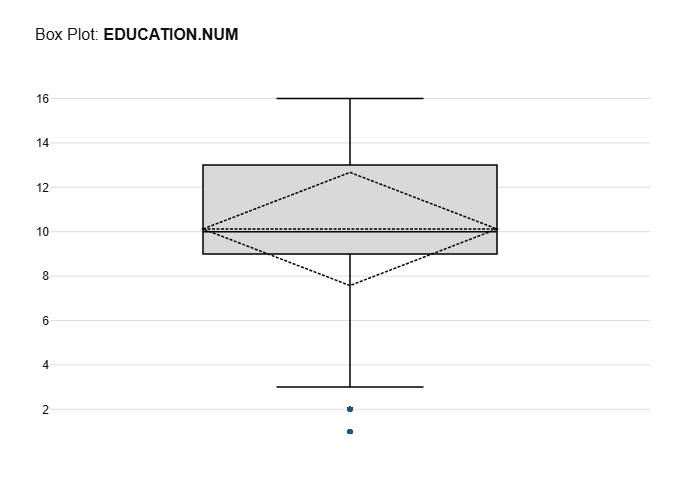
\includegraphics[width=0.8\linewidth]{figures/educationnum_b.png}
    \caption{\textbf{Boxplot di Education Num.} il 50\% dei casi è contenuto tra 9 e 13. Il grafico conferma una scarsa propensione in bassa istruzione della popolazione}
    \label{fig:edu_b.png}
\end{figure}

\noindent
\textbf{Interpretazione:}
\begin{itemize}
    \item La media leggermente superiore a 10 indica che il campione medio possiede un livello di istruzione superiore al diploma.
    \item L'asimmetria negativa (-0.30) riflette la concentrazione della popolazione verso livelli di istruzione medio-alti.
    \item \textbf{Relazione bivariata:} Si conferma come uno dei predittori più forti; la differenza del 33.33\% nella mediana (+3 anni di studio) è un segnale predittivo critico.
\end{itemize}

\newpage
% --- ANALISI DETTAGLIATA CAPITAL.GAIN ---
\subsubsection{Analisi di \texttt{capital.gain}}

\begin{table}[H]
    \centering
    \footnotesize
    \caption{Dettaglio \texttt{capital.gain} per gruppo di reddito e analisi del Delta}
    
    \textbf{Tabella A: Statistiche per Gruppo} \\
    \begin{tabular}{lrrrrrrrr}
        \toprule
        \textbf{income} & \textbf{Conteggio} & \textbf{Media} & \textbf{Mediana} & \textbf{Dev. Std} & \textbf{Min} & \textbf{Max} & \textbf{IQR} & \textbf{Skew} \\
        \midrule
        $\leq 50K$ & 22,633.00 & 149.03 & 0.00 & 936.82 & 0.00 & 41,310.00 & 0.00 & 17.41 \\
        $> 50K$ & 7,506.00 & 3,938.73 & 0.00 & 14,387.83 & 0.00 & 99,999.00 & 0.00 & 5.91 \\
        \bottomrule
    \end{tabular}

    \vspace{0.4cm}
    
    \textbf{Tabella B: Delta Report ($>50K$ vs $\leq 50K$)} \\
    \begin{tabular}{clrrrr}
        \toprule
        \textbf{ID} & \textbf{Metrica} & \textbf{$\leq 50K$ (Base)} & \textbf{$> 50K$ (Confronto)} & \textbf{Diff. Assoluta} & \textbf{Diff. \%} \\
        \midrule
        0 & Media & 149.03 & 3,938.73 & +3,789.70 & +2542.87\% \\
        1 & Mediana & 0.00 & 0.00 & +0.00 & +0.00\% \\
        2 & Dev. Std & 936.82 & 14,387.83 & +13,451.02 & +1435.82\% \\
        3 & IQR & 0.00 & 0.00 & +0.00 & +0.00\% \\
        \bottomrule
    \end{tabular}
\end{table}

\begin{figure}[H]
    \centering
    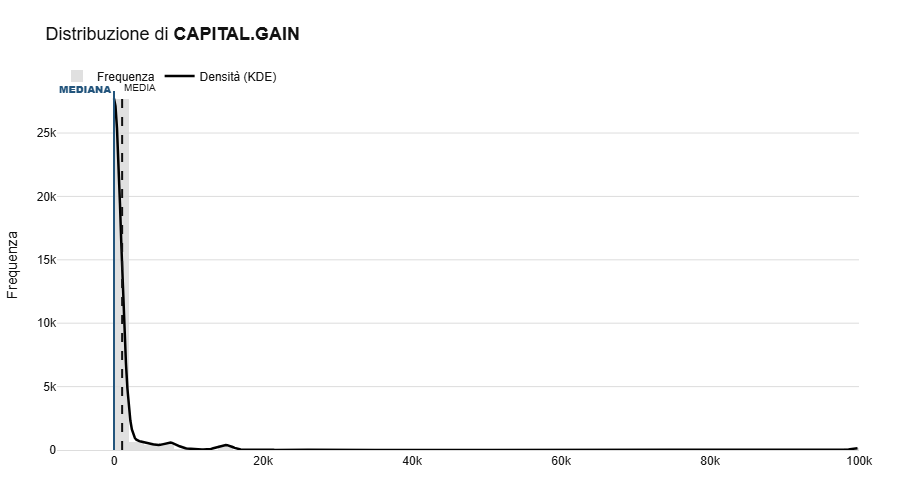
\includegraphics[width=1\linewidth]{figures/capitalgain1.png}
    \caption{\textbf{Distribuzione di Capital Gain.} La massa di osservazioni a zero domina completamente
la visualizzazione}
    \label{fig:uni_cap_gain}
\end{figure}

\begin{figure}[H]
    \centering
    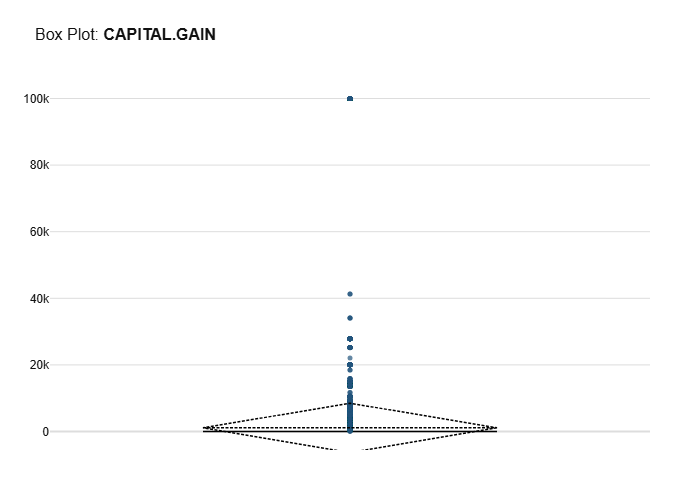
\includegraphics[width=0.8\linewidth]{figures/capitalgain_b.png}
    \caption{\textbf{Boxplot di Capital Gain.} Quasi la totalità dei valori è a zero. La presenza di outlier estremi è evidente con il max di 99,999.}
    \label{fig:capitalgain_b.png}
\end{figure}

\noindent
\textbf{Interpretazione:}
\begin{itemize}
    \item Persiste la caratteristica patologica di \textit{zero-inflation} (Mediana e Moda = 0).
    \item La kurtosis estrema (+153.55) indica una distribuzione quasi degenere su zero con eventi rarissimi di valore altissimo.
    \item \textbf{Trasformazione necessaria:} La differenza del +2542\% nella media tra le classi indica che, sebbene raro, il guadagno di capitale è quasi esclusivo della classe ad alto reddito.
\end{itemize}

\newpage
% --- ANALISI DETTAGLIATA CAPITAL.LOSS ---
\subsubsection{Analisi di \texttt{capital.loss}}

\begin{table}[H]
    \centering
    \footnotesize
    \caption{Dettaglio \texttt{capital.loss} per gruppo di reddito e analisi del Delta}
    
    \textbf{Tabella A: Statistiche per Gruppo} \\
    \begin{tabular}{lrrrrrrrr}
        \toprule
        \textbf{income} & \textbf{Conteggio} & \textbf{Media} & \textbf{Mediana} & \textbf{Dev. Std} & \textbf{Min} & \textbf{Max} & \textbf{IQR} & \textbf{Skew} \\
        \midrule
        $\leq 50K$ & 22,633.00 & 53.50 & 0.00 & 310.41 & 0.00 & 4,356.00 & 0.00 & 5.95 \\
        $> 50K$ & 7,506.00 & 193.80 & 0.00 & 592.90 & 0.00 & 3,683.00 & 0.00 & 2.80 \\
        \bottomrule
    \end{tabular}

    \vspace{0.4cm}
    
    \textbf{Tabella B: Delta Report ($>50K$ vs $\leq 50K$)} \\
    \begin{tabular}{clrrrr}
        \toprule
        \textbf{ID} & \textbf{Metrica} & \textbf{$\leq 50K$ (Base)} & \textbf{$> 50K$ (Confronto)} & \textbf{Diff. Assoluta} & \textbf{Diff. \%} \\
        \midrule
        0 & Media & 53.50 & 193.80 & +140.30 & +262.26\% \\
        1 & Mediana & 0.00 & 0.00 & +0.00 & +0.00\% \\
        2 & Dev. Std & 310.41 & 592.90 & +282.49 & +91.00\% \\
        3 & IQR & 0.00 & 0.00 & +0.00 & +0.00\% \\
        \bottomrule
    \end{tabular}
\end{table}

\begin{figure}[H]
    \centering
    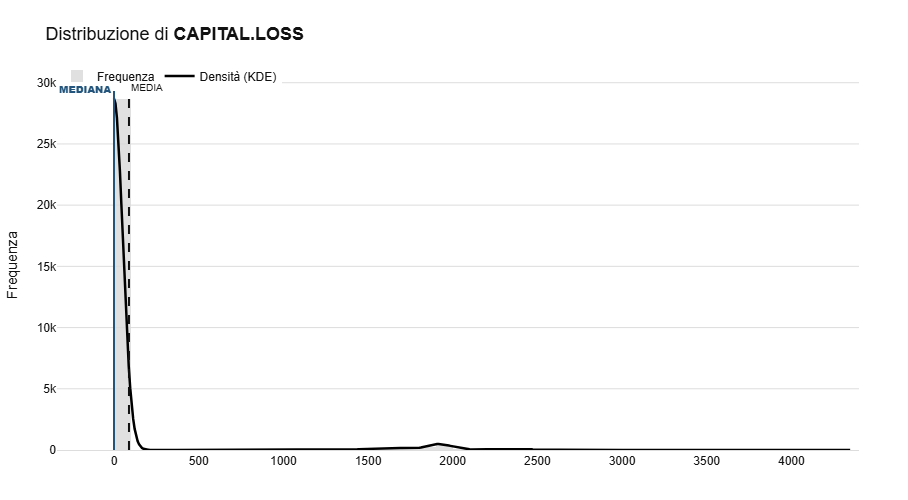
\includegraphics[width=1\linewidth]{figures/capitalloss1.png}
    \caption{\textbf{Distribuzione di Capital Loss.} Analogamente al gain, la variabile è dominata da zeri con una coda destra per investimenti falliti.}
    \label{fig:uni_cap_loss}
\end{figure}

\begin{figure}[H]
    \centering
    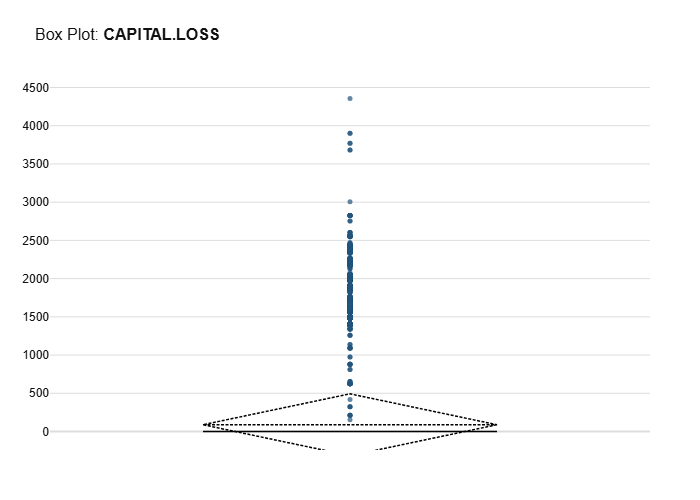
\includegraphics[width=1\linewidth]{figures/capitalloss_b.png}
    \caption{\textbf{Boxplot di Capital Loss.} Analogamente al gain, la variabile è dominata da zeri con una outlier.}
    \label{fig:capitalloss_b.png}
\end{figure}

\noindent
\textbf{Interpretazione:}
\begin{itemize}
    \item Comportamento analogo a \texttt{capital.gain}, con una prevalenza massiccia di zeri.
    \item \textbf{Implicazione:} La variabile è sparsa ma informativa; la differenza del 262\% nella media suggerisce che chi possiede asset finanziari (e subisce perdite) appartiene più frequentemente alla classe $>50K$.
\end{itemize}

\newpage
% --- ANALISI DETTAGLIATA HOURS.PER.WEEK ---
\subsubsection{Analisi di \texttt{hours.per.week}}

\begin{table}[H]
    \centering
    \footnotesize
    \caption{Dettaglio \texttt{hours.per.week} per gruppo di reddito e analisi del Delta}
    
    \textbf{Tabella A: Statistiche per Gruppo} \\
    \begin{tabular}{lrrrrrrrr}
        \toprule
        \textbf{income} & \textbf{Conteggio} & \textbf{Media} & \textbf{Mediana} & \textbf{Dev. Std} & \textbf{Min} & \textbf{Max} & \textbf{IQR} & \textbf{Skew} \\
        \midrule
        $\leq 50K$ & 22,633.00 & 39.35 & 40.00 & 11.95 & 1.00 & 99.00 & 2.00 & 0.30 \\
        $> 50K$ & 7,506.00 & 45.71 & 40.00 & 10.74 & 1.00 & 99.00 & 10.00 & 0.85 \\
        \bottomrule
    \end{tabular}

    \vspace{0.4cm}
    
    \textbf{Tabella B: Delta Report ($>50K$ vs $\leq 50K$)} \\
    \begin{tabular}{clrrrr}
        \toprule
        \textbf{ID} & \textbf{Metrica} & \textbf{$\leq 50K$ (Base)} & \textbf{$> 50K$ (Confronto)} & \textbf{Diff. Assoluta} & \textbf{Diff. \%} \\
        \midrule
        0 & Media & 39.35 & 45.71 & +6.36 & +16.15\% \\
        1 & Mediana & 40.00 & 40.00 & +0.00 & +0.00\% \\
        2 & Dev. Std & 11.95 & 10.74 & -1.21 & -10.13\% \\
        3 & IQR & 2.00 & 10.00 & +8.00 & +400.00\% \\
        \bottomrule
    \end{tabular}
\end{table}

\begin{figure}[H]
    \centering
    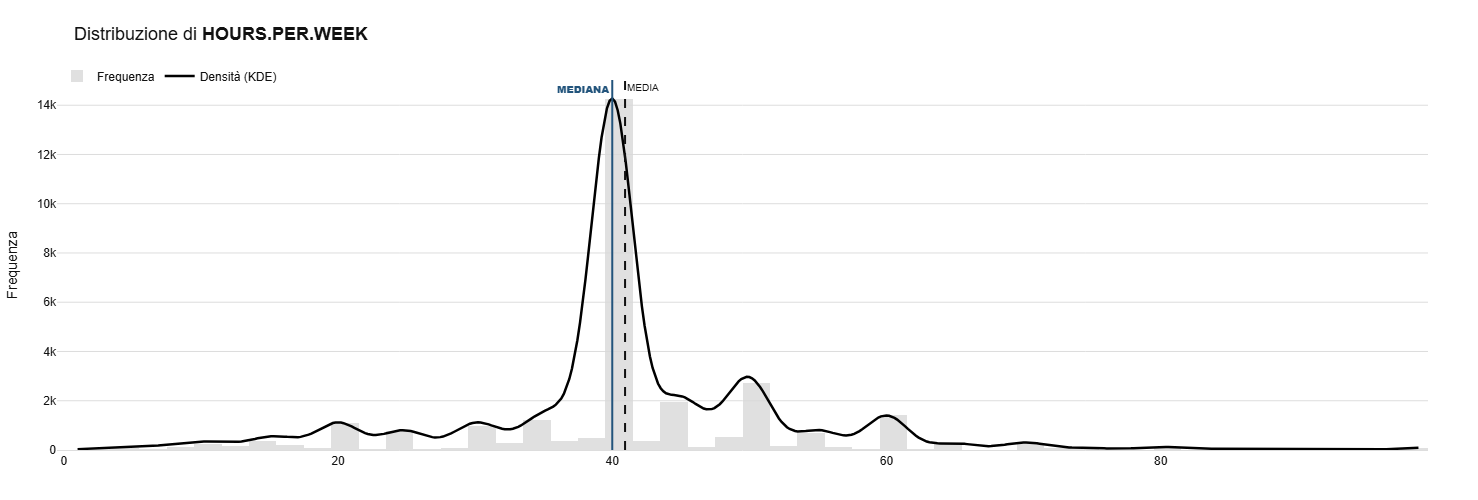
\includegraphics[width=1\linewidth]{figures/hoursperweek1.png}
    \caption{\textbf{Distribuzione di Hours per Week.} Si nota una concentrazione estrema sulla moda di 40 ore per entrambe le classi.}
    \label{fig:uni_hours}
\end{figure}

\begin{figure}[H]
    \centering
    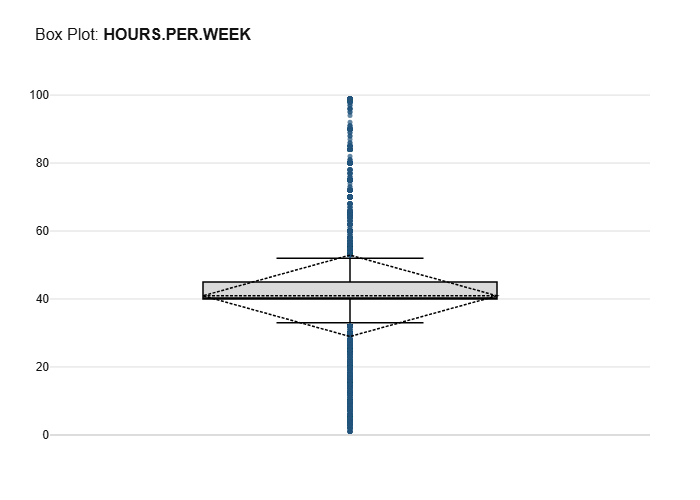
\includegraphics[width=0.8\linewidth]{figures/hoursperweek_b.png}
    \caption{\textbf{Boxplot di Hours per Week.} Il grafico mostra una bassa dispersione dei valori, si concentrano attorno dalle 40 ore settimanali. Si notano diversi outlier}
    \label{fig:hoursperweek_b.png}
\end{figure}

\noindent
\textbf{Interpretazione:}
\begin{itemize}
    \item La media di 45.71 ore per la classe $>50K$ rispetto alle 39.35 della classe base suggerisce la correlazione tra impegno orario e reddito.
    \item L'esplosione dell'IQR (+400\%) nella classe superiore indica una maggiore variabilità: i redditi alti lavorano o le canoniche 40 ore o significativamente di più (code pesanti).
    \item \textbf{Stabilità:} È la variabile continua più regolare del dataset, con una forte concentrazione sulla "settimana lavorativa standard".
\end{itemize}

\subsection{Analisi Bivariata: Boxplot e Pairplot}

\begin{figure}[H]
    \centering
    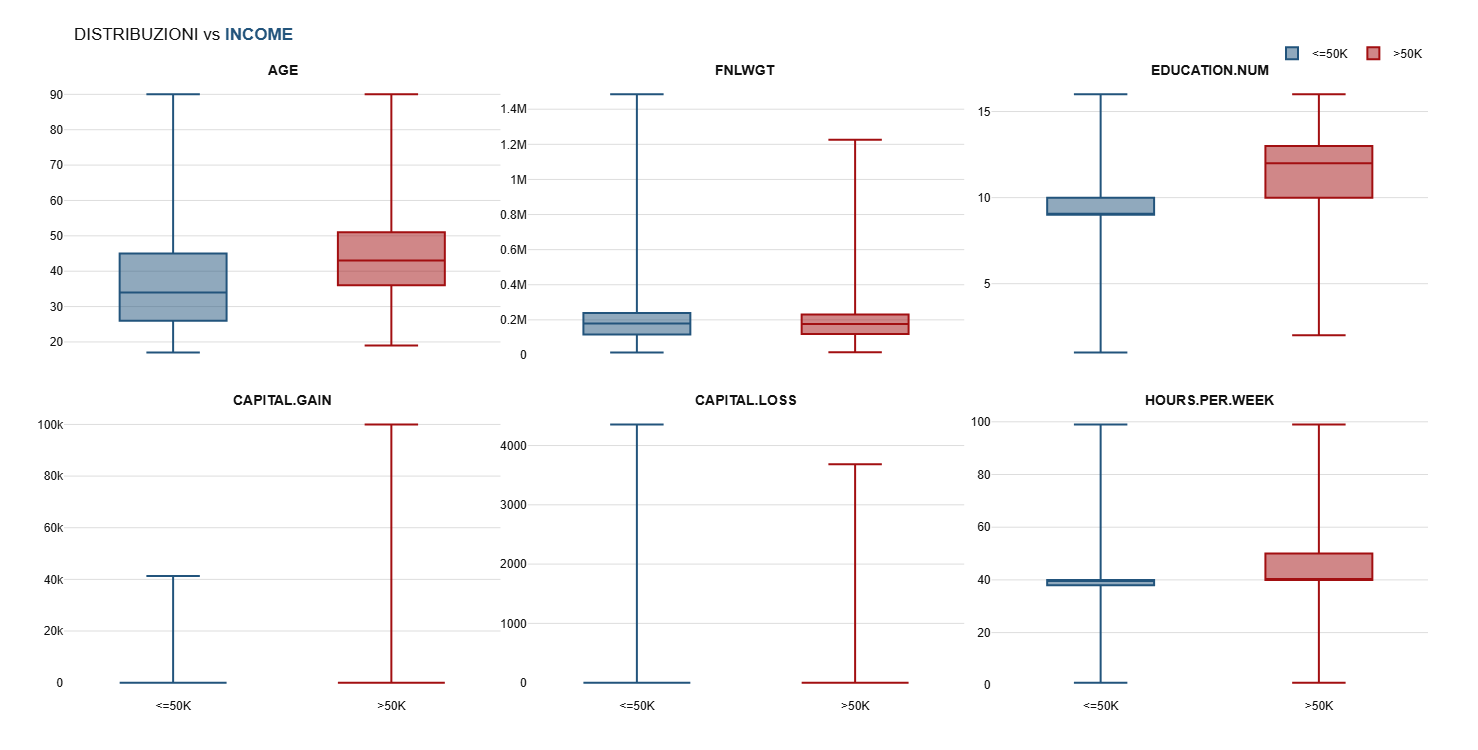
\includegraphics[width=1\linewidth]{figures/boxplot_confornti.png}
    \caption{\textbf{Comparazione dei boxplot delle categorie numeriche per classe.} La differenza più marcata si osserva in \texttt{education.num}, mentre \texttt{fnlwgt} mostra una sovrapposizione quasi totale.}
    \label{fig:boxplot_confronti.png}
\end{figure}

\begin{figure}[H]
    \centering
    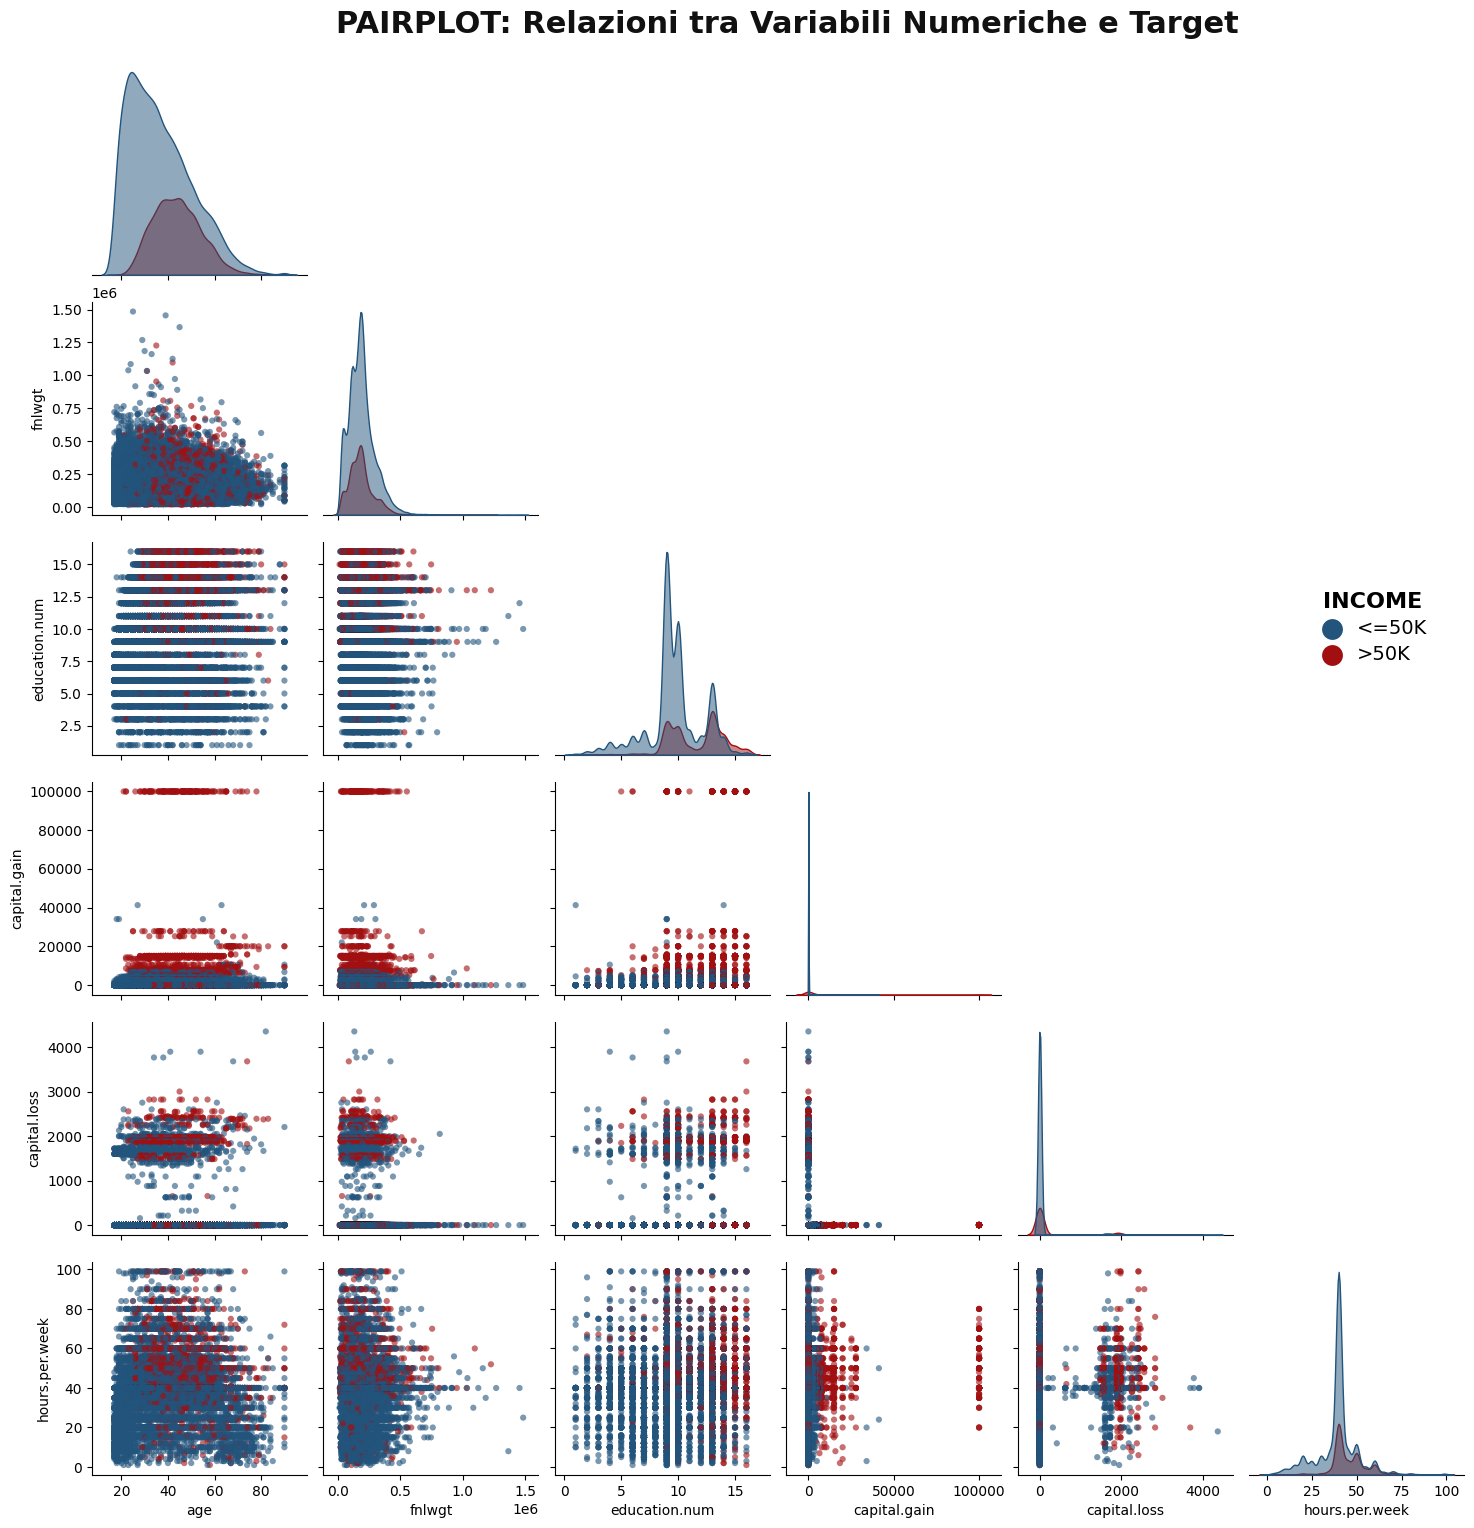
\includegraphics[width=1.01\linewidth]{figures/pairplot.png}
    \caption{\textbf{Pairplot.}}
    \label{fig:pairplot.png}
\end{figure}

\newpage
\subsection{Analisi delle Correlazioni tra Feature Numeriche}

\begin{figure}[H]
    \centering
    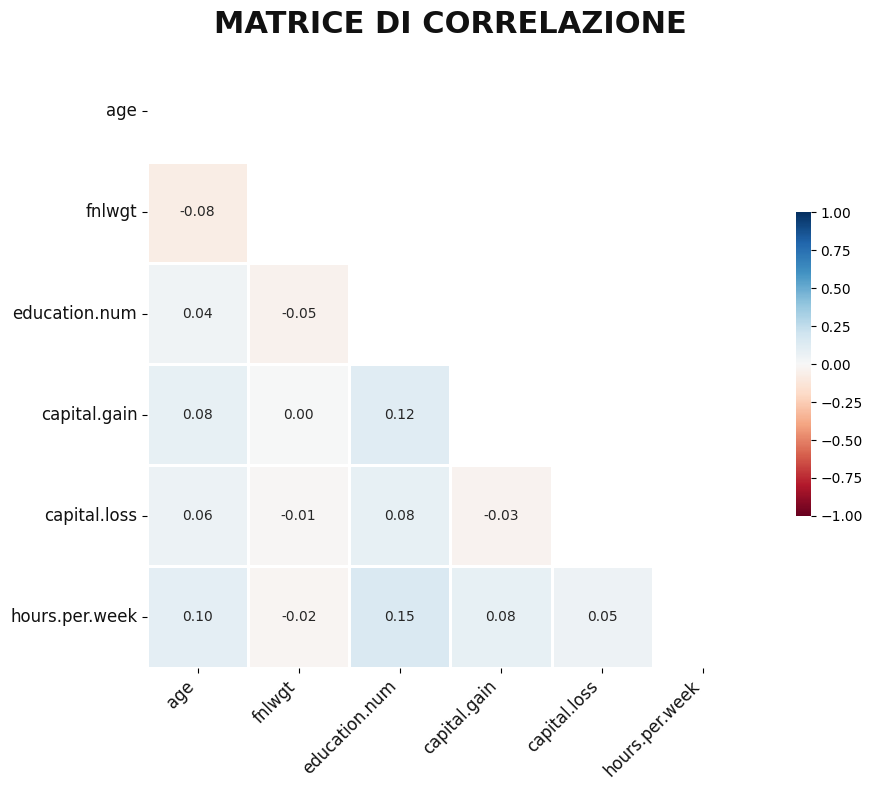
\includegraphics[width=0.8\linewidth]{figures/matrice_correlazione.png}
    \caption{\textbf{Matrice di Correlazione di Pearson.} I valori ridotti (max $r=0.15$) evidenziano un'assenza di multicollinearità e una forte indipendenza lineare tra le feature.}
    \label{fig:matrice_correlazione.png}
\end{figure}

Al fine di identificare potenziali ridondanze informative e valutare il rischio di multicollinearità, è stata analizzata la matrice di correlazione per le variabili numeriche.
I risultati evidenziano uno scenario di forte indipendenza lineare tra i predittori. Come si evince dai dati, non emerge alcun cluster di variabili fortemente correlate. Nello specifico:

\begin{itemize}
    \item \textbf{Assenza di Multicollinearità:} Il coefficiente massimo registrato nell'intera matrice è pari a $r = 0.15$. Tale valore è inferiore alle soglie di allarme tipicamente considerate critiche in letteratura ($|r| > 0.85$), garantendo che nessuna feature numerica sia una combinazione lineare delle altre.
    
    \item \textbf{Relazioni Deboli ma Interpretabili:} Anche le associazioni logicamente attese risultano deboli. Ad esempio, la correlazione tra (\texttt{education.num}) e (\texttt{capital.gain}) si attesta su un modesto $r = 0.12$. Questo suggerisce che, sebbene esista una lieve tendenza positiva, le due variabili catturano aspetti diversi del profilo socio-economico dell'individuo.
    
    \item \textbf{Neutralità del Peso Campionario:} La variabile \texttt{fnlwgt} mostra correlazioni quasi nulle con tutte le altre feature (valori compresi tra $-0.08$ e $0.00$). Ciò conferma empiricamente che il peso statistico assegnato dal censimento è ortogonale alle caratteristiche demografiche del soggetto.
\end{itemize}

\noindent
\textbf{Implicazioni per la modellazione:} 
Data l'assenza di ridondanza informativa tra le variabili, non si ritiene necessario applicare tecniche di feature selection basate sulla rimozione di collinearità.
    \newpage
    \setcounter{figure}{0}
\renewcommand{\thefigure}{A.\arabic{figure}}
\setcounter{table}{0}
\renewcommand{\thetable}{A.\arabic{table}}


\section{Inferenza Statistica e Feature Selection}
\label{app:stat_inference}

La presente appendice formalizza il framework metodologico adottato per l'analisi esplorativa e la selezione delle variabili. Il protocollo è stato progettato per garantire la robustezza delle stime in presenza di grandi campioni ($N > 30.000$) e per mitigare il rischio di scoperte false positive (Type I errors) derivanti da test di ipotesi multipli.

\subsection{Verifica delle Assunzioni Distributive}

La validità dei test parametrici è subordinata al rispetto delle assunzioni di normalità e omoschedasticità. Data la sensibilità dei test di bontà dell'adattamento (*goodness-of-fit*) alla dimensione campionaria, è stata implementata una strategia adattiva.

\subsection{Test di Normalità Ibrido}
Per la verifica dell'ipotesi nulla di normalità $H_0: F(x) \sim \mathcal{N}(\mu, \sigma^2)$, è stato adottato un criterio decisionale basato sulla numerosità campionaria $N$:

\begin{itemize}
    \item \textbf{Per $N < 5000$ (Shapiro-Wilk):} Si utilizza la statistica $W$ di Shapiro-Wilk, che valuta la correlazione tra i dati ordinati e i punteggi normali attesi. Questo test offre la massima potenza statistica per campioni ridotti o medi.
    \item \textbf{Per $N \ge 5000$ (Jarque-Bera):} Al crescere di $N$, il test di Shapiro-Wilk tende a rifiutare $H_0$ anche per deviazioni trascurabili dalla normalità (paradosso della potenza eccessiva). In questo regime asintotico, si adotta il test di Jarque-Bera, che si basa sui momenti terzi e quarti della distribuzione empirica (skewness $S$ e kurtosis $K$):
    \begin{equation}
        JB = \frac{N}{6} \left( S^2 + \frac{(K-3)^2}{4} \right)
    \end{equation}
    Il test verifica asintoticamente se i momenti campionari coincidono con quelli di una distribuzione normale ($S=0, K=3$).
\end{itemize}

\begin{figure}[H]
    \centering
    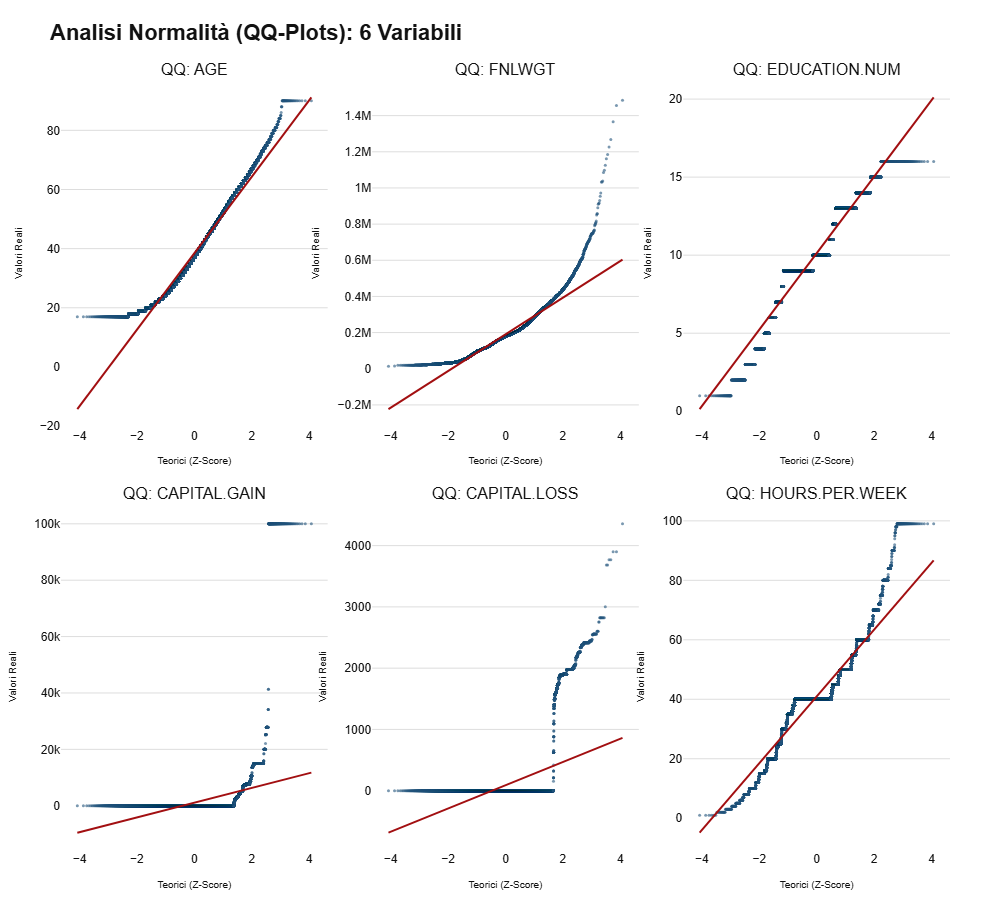
\includegraphics[width=1\linewidth]{figures/qq.png}
    \caption{\textbf{QQ Plot}  Nel complesso, l’analisi evidenzia che la maggior parte delle variabili non segue una distribuzione normale, suggerendo l’eventuale necessità di trasformazioni o l’utilizzo di metodi statistici robusti o non parametrici nelle analisi successive.}
    \label{fig:qq.png}
\end{figure}

\subsection{Omoschedasticità}
L'assunzione di omogeneità delle varianze tra i gruppi è stata verificata mediante il \textbf{test di Levene} centrato sulla mediana (metodo Brown-Forsythe). Tale approccio è preferito al test di Bartlett in quanto significativamente più robusto alle violazioni della normalità distributiva.

\subsection{Test di Ipotesi e Correzione FDR}

La selezione del test statistico per valutare la relazione tra le feature $X_i$ e la variabile target $Y$ avviene dinamicamente secondo l'albero decisionale riportato in Tabella \ref{tab:test}.

\begin{table}[H]
\centering
\begin{tabular}{lccc}
\toprule
\textbf{Tipologia $X_i$} & \textbf{Normalità} & \textbf{Omoschedasticità} & \textbf{Test Statistico} \\
\midrule
Categorica & - & - & $\chi^2$ di Pearson \\
Numerica & Sì & Sì & $t$-test di Student / ANOVA \\
Numerica & Sì & No & $t$-test di Welch / Welch ANOVA \\
Numerica & No & - & Mann-Whitney $U$ / Kruskal-Wallis \\
\bottomrule
\end{tabular}
\caption{Matrice decisionale per la selezione dei test di ipotesi.}
\label{tab:test}
\end{table}

\subsection{Controllo del False Discovery Rate (FDR)}
Conducendo $m$ test simultanei (uno per ogni feature), la probabilità di commettere almeno un errore di I tipo (FWER) aumenta drasticamente. Per ovviare a ciò senza incorrere nell'eccessivo conservatorismo della correzione di Bonferroni, si è applicata la procedura di \textbf{Benjamini-Hochberg}.
\noindent
Dato l'insieme dei $p$-value ordinati $p_{(1)} \le p_{(2)} \le \dots \le p_{(m)}$, la procedura identifica il più grande indice $k$ tale che:
\begin{equation}
    p_{(k)} \le \frac{k}{m} \alpha
\end{equation}
Tutti i test con $p$-value $p_{(i)} \le p_{(k)}$ vengono dichiarati significativi, controllando il tasso atteso di false scoperte al livello $\alpha=0.05$.

\subsection{Stima della Dimensione dell'Effetto (Effect Size)}

La sola significatività statistica ($p < \alpha$) non implica rilevanza pratica, specialmente in presenza di grandi dataset dove differenze infinitesimali risultano statisticamente significative. L'analisi è stata integrata con metriche di \textit{Effect Size} standardizzate.

\subsection{Vargha-Delaney $\hat{A}_{12}$ (Non-Parametrico)}
Per le variabili numeriche che non soddisfano l'assunzione di normalità (e.g., analizzate con Mann-Whitney $U$), è stata calcolata la misura di \textit{Stochastic Superiority} $\hat{A}_{12}$ di Vargha e Delaney. Questa metrica stima la probabilità che un valore estratto casualmente da un gruppo sia maggiore di un valore estratto dall'altro:
\begin{equation}
    \hat{A}_{12} = \frac{R_1/n_1 - (n_1+1)/2}{n_2}
\end{equation}
dove $R_1$ è la somma dei ranghi del primo gruppo. L'interpretazione si basa sulla distanza dall'ipotesi nulla (0.5):
\begin{itemize}
    \item Trascurabile: $| \hat{A}_{12} - 0.5 | < 0.06$
    \item Piccolo: $0.06 \le | \hat{A}_{12} - 0.5 | < 0.14$
    \item Medio: $0.14 \le | \hat{A}_{12} - 0.5 | < 0.21$
    \item Grande: $| \hat{A}_{12} - 0.5 | \ge 0.21$
\end{itemize}

\subsection{Cramer's $V$ (Categorico)}
Per le tabelle di contingenza derivanti dal test $\chi^2$, l'intensità dell'associazione è stata misurata tramite la V di Cramer, normalizzando la statistica $\chi^2$ rispetto alla dimensione campionaria $N$ e ai gradi di libertà minimi ($q = \min(r-1, c-1)$):
\begin{equation}
    V = \sqrt{\frac{\chi^2}{N \cdot q}}
\end{equation}

\subsection{Algoritmo di Feature Selection}

Sulla base delle inferenze prodotte, è stato definito un algoritmo di selezione volto a identificare i predittori ottimali per la modellazione successiva. Una feature viene candidata all'esclusione se soddisfa almeno una delle seguenti condizioni critiche:

\begin{enumerate}
    \item \textbf{Criterio di Sparsità:} Percentuale di valori mancanti $> 60\%$.
    \item \textbf{Criterio di Varianza:} Varianza nulla (feature costante).
    \item \textbf{Criterio di Inferenza (Rumore):} $p\text{-value}_{adj} > 0.05$.
    \item \textbf{Criterio di Rilevanza (Effect Size):} La feature risulta statisticamente significativa ma l'effetto stimato è classificato come "Trascurabile" (e.g., Vargha-Delaney $\hat{A}_{12} \approx 0.5$).
\end{enumerate}

\noindent
L'applicazione di tale protocollo al dataset in esame ha evidenziato la non significatività della variabile \texttt{fnlwgt} ($p_{adj}=0.08$) e la scarsa rilevanza pratica di \texttt{capital.loss} ($\hat{A}_{12}=0.466$, effetto trascurabile), suggerendone l'esclusione per parsimonia del modello.

    \newpage
    % Reset dei contatori per l'appendice
\setcounter{figure}{0}
\renewcommand{\thefigure}{A.\arabic{figure}}
\setcounter{table}{0}
\renewcommand{\thetable}{A.\arabic{table}}

\section{Feature Engineering e Riduzione della Dimensionalità}
\label{app:feature_engineering}

Questa sezione documenta le trasformazioni applicate allo spazio delle feature originali al fine di migliorarne la qualità informativa e la trattabilità computazionale. L'attenzione si è focalizzata sulla gestione delle variabili categoriche ad alta cardinalità che presentano sfide critiche legate alla sparsità e alla stabilità statistica delle stime.

\subsection{Gestione della Cardinalità: Il caso \texttt{native.country}}

L'analisi preliminare della variabile \texttt{native.country} ha evidenziato una distribuzione altamente sbilanciata e frammentata. La variabile originale presentava numerosi livelli (paesi) con frequenze assolute trascurabili ($n_i < 50$), configurando un problema di \textit{Sparse Classes}.

Mantenere tale granularità comporterebbe due rischi principali in fase di modellazione:
\begin{enumerate}
    \item \textbf{Esposizione alla "Curse of Dimensionality":} L'applicazione di tecniche di codifica come il One-Hot Encoding genererebbe una matrice sparsa con dozzine di colonne quasi vuote.
    \item \textbf{Instabilità dell'Inferenza:} I coefficienti stimati per le categorie rare sarebbero caratterizzati da varianza elevata e scarsa generalizzabilità (rischio di overfitting su specifici pattern di rumore).
\end{enumerate}

\subsection{Strategia di Aggregazione (Binning)}
Per mitigare tali criticità, è stata implementata una strategia di riduzione della dimensionalità basata sull'aggregazione semantica. La variabile è stata trasformata in una feature binaria \texttt{native\_region} secondo la seguente logica di mappatura $f(x)$:

\begin{equation}
    f(x) = 
    \begin{cases} 
    \text{'USA'} & \text{se } x = \text{'United-States'} \\
    \text{'Other'} & \text{altrimenti}
    \end{cases}
\end{equation}

\noindent
Tale trasformazione assume che la distinzione discriminante principale nel dataset (Census Income, di natura socio-economica statunitense) risieda nella dicotomia tra nativi e non nativi, piuttosto che nelle specificità del singolo paese di origine estero.

\subsection{Analisi della Distribuzione Post-Processing}

A seguito della trasformazione, è stata condotta un'analisi della frequenza per valutare il nuovo assetto distributivo della feature \texttt{native\_region}.

\begin{figure}[H]
    \centering
    % Placeholder per l'immagine generata dal codice Python
    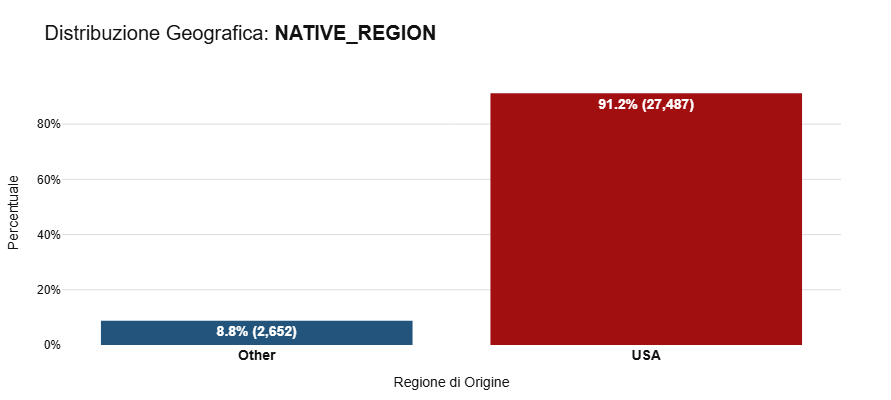
\includegraphics[width=1\textwidth]{figures/bilanciamento_country.png} 
    \caption{Distribuzione delle frequenze per la feature ingegnerizzata \texttt{native\_region}. Si evidenzia la netta predominanza della classe 'USA'.}
    \label{fig:bilanciamento_country.png}
\end{figure}

\noindent
L'analisi quantitativa (Figura \ref{fig:bilanciamento_country.png}) evidenzia che la categoria 'USA' assorbe la vasta maggioranza delle osservazioni ($>90\%$). Sebbene l'operazione abbia risolto il problema della sparsità, ha introdotto (o meglio, cristallizzato) un forte sbilanciamento di classe.

\subsection{Implicazioni per la Modellazione}
La concentrazione di massa sulla classe 'USA' riduce la varianza della feature, limitandone potenzialmente il potere predittivo (\textit{Information Gain}). Una variabile con una categoria dominante al $90\%+$ tende ad approssimarsi a una costante.
Tuttavia, il mantenimento della distinzione 'USA' vs 'Other' è ritenuto preferibile alla rimozione totale della variabile, in quanto permette al modello di catturare eventuali bias sistemici legati allo status di immigrazione, pur in un contesto di bassa entropia.

\newpage
    \newpage
    % Reset dei contatori per l'appendice
\setcounter{figure}{0}
\renewcommand{\thefigure}{A.\arabic{figure}}
\setcounter{table}{0}
\renewcommand{\thetable}{A.\arabic{table}}

\section{Preprocessing del Target e Partitioning}
\label{app:data_splitting}

In questa sezione si descrivono le operazioni preliminari di codifica della variabile dipendente e la strategia di suddivisione del dataset (\textit{Data Splitting}) adottata per la fase di addestramento e validazione.

\subsection{Codifica della Variabile Target}

La variabile target originale \texttt{income}, di natura categorica nominale, è stata sottoposta a una procedura di pulizia e mappatura binaria per renderla idonea agli algoritmi di classificazione.
Al fine di garantire la robustezza del parsing contro eventuali artefatti di formattazione (e.g., spaziature o punteggiatura residua come \texttt{'<=50K.'}), è stata applicata una funzione di normalizzazione delle stringhe prima della codifica.
\noindent
La trasformazione è definita dalla seguente mappatura $M: \mathcal{Y}_{raw} \to \{0, 1\}$:
\begin{equation}
    y_i = 
    \begin{cases} 
    0 & \text{se } \texttt{income}_i \in \{\text{'<=50K'}\} \\
    1 & \text{se } \texttt{income}_i \in \{\text{'>50K'}\}
    \end{cases}
\end{equation}
La classe positiva ($y=1$) identifica gli individui con reddito superiore alla soglia, costituendo il target di interesse per la predizione.

\subsection{Strategia di Partitioning (Stratified Hold-out)}

Il dataset processato ($N=30.139$) è stato suddiviso in due sottoinsiemi disgiunti secondo un rapporto 80/20:
\begin{itemize}
    \item \textbf{Training Set ($S_{train}$):} 80\% dei dati ($n_{train} = 24.111$), utilizzato per la stima dei parametri del modello.
    \item \textbf{Test Set ($S_{test}$):} 20\% dei dati ($n_{test} = 6.028$), riservato esclusivamente per la valutazione delle performance su dati non osservati (\textit{unseen data}).
\end{itemize}

Per garantire la riproducibilità dell'esperimento, è stato fissato un \textit{seed} globale (\texttt{random\_state=42}).

\subsection{Campionamento Stratificato}
Dato il moderato sbilanciamento delle classi nel dataset originale (tasso di positività $\approx 24.9\%$), un campionamento casuale semplice (\textit{Simple Random Sampling}) avrebbe potuto introdurre bias campionari, alterando le probabilità a priori delle classi nei due sottoinsiemi.

\noindent
È stato pertanto adottato lo \textbf{Stratified Sampling}, vincolando lo split a preservare la proporzione originale delle classi:
\begin{equation}
    P(y=1 | S_{train}) \approx P(y=1 | S_{test}) \approx P(y=1 | S_{total})
\end{equation}

\noindent
La verifica a posteriori (Tabella \ref{tab:split_verify}) conferma l'efficacia della stratificazione, con una divergenza ($\Delta$) tra le distribuzioni del Training e del Test set inferiore allo $0.01\%$, garantendo che la valutazione sul test set sia rappresentativa della distribuzione reale.

\begin{table}[h]
\centering
\begin{tabular}{lccc}
\toprule
\textbf{Classe} & \textbf{Training Set \%} & \textbf{Test Set \%} & \textbf{Delta ($\Delta$)} \\
\midrule
0 ($\le$50K) & 75.0944\% & 75.0995\% & 0.0052\% \\
1 ($>$50K) & 24.9056\% & 24.9005\% & 0.0052\% \\
\bottomrule
\end{tabular}
\caption{Verifica della distribuzione delle classi post-split.}
\label{tab:split_verify}
\end{table}

    \newpage
    % Reset dei contatori per l'appendice
\setcounter{figure}{0}
\renewcommand{\thefigure}{A.\arabic{figure}}
\setcounter{table}{0}
\renewcommand{\thetable}{A.\arabic{table}}

\section{Feature Encoding e Costruzione del Dataset}
\label{app:feature_encoding}

In questa sezione si descrive la procedura di trasformazione delle variabili categoriche in rappresentazioni numeriche idonee per l'elaborazione algoritmica, nonché la ricomposizione finale delle matrici di design.

\subsection{Identificazione e Segregazione dei Tipi di Dato}

Preliminarmente, lo spazio delle feature $\mathcal{X}$ è stato partizionato in due sottoinsiemi disgiunti in base alla tipologia del dato, utilizzando l'insieme di addestramento $X_{train}$ come unico riferimento per evitare contaminazioni informative (\textit{Look-ahead Bias}):

\begin{itemize}
    \item \textbf{Sottoinsieme Numerico ($\mathcal{X}_{num}$):} Include 5 variabili continue o discrete ordinali. Queste variabili non richiedono codifica ma saranno oggetto di successiva standardizzazione.
    \item \textbf{Sottoinsieme Categorico ($\mathcal{X}_{cat}$):} Include 8 variabili nominali che necessitano di una trasformazione in vettori numerici.
\end{itemize}

\subsection{One-Hot Encoding}

Per la codifica delle variabili in $\mathcal{X}_{cat}$, è stata adottata la tecnica del \textbf{One-Hot Encoding}. Tale metodo trasforma ogni variabile categorica con $k$ livelli distinti in $k$ variabili binarie (dummy variables) $\{d_1, \dots, d_k\}$, dove $d_i \in \{0, 1\}$.
Nonostante l'incremento della dimensionalità, l'OHE è preferibile all'\textit{Ordinal Encoding} per variabili nominali prive di ordinamento intrinseco, in quanto evita di introdurre relazioni di distanza spuria tra le categorie (e.g., assumere che $2 \times \text{Divorced} = \text{Married}$).

\subsection{Configurazione e Robustezza}
Il trasformatore è stato configurato con i seguenti parametri critici per garantire la robustezza in produzione:
\begin{itemize}
    \item \textbf{Addestramento Esclusivo:} L'apprendimento del mapping categorie-colonne (\texttt{fit}) è avvenuto esclusivamente su $X_{train}$.
    \item \textbf{Gestione Unknown Categories:} È stato abilitato il parametro \texttt{handle\_unknown='ignore'}. Qualora nel Test Set compaia una categoria non osservata durante il training, l'encoder genererà un vettore di zeri (tutte le dummy a 0) anziché sollevare un'eccezione, garantendo la continuità operativa del modello.
\end{itemize}

\subsection{Trasformazione e Integrità Dimensionale}

L'applicazione dell'encoder ha comportato un'espansione dello spazio delle feature da 13 a 64 dimensioni.
La trasformazione $T(\cdot)$ applicata a un generico vettore di input $\mathbf{x}$ è definita come la concatenazione delle componenti numeriche originali e delle componenti categoriche codificate:

\begin{equation}
    \mathbf{x}_{ready} = \left[ \mathbf{x}_{num} \parallel \text{OHE}(\mathbf{x}_{cat}) \right]
\end{equation}

\noindent
La procedura ha generato 59 nuove feature binarie a partire dalle 8 categoriche originali.
La verifica di integrità finale (Tabella \ref{tab:encoding_dims}) conferma la coerenza dimensionale tra i set e l'assenza di valori mancanti (\textit{NaN}) introdotti durante il processo di merge, che è stato eseguito preservando rigorosamente l'allineamento degli indici.

\newpage
\begin{table}[h]
\centering
\begin{tabular}{lccc}
\toprule
\textbf{Dataset} & \textbf{Righe ($N$)} & \textbf{Colonne ($D$)} & \textbf{Stato} \\
\midrule
Training Set ($X_{train}$) & 24.111 & 64 & Ready \\
Test Set ($X_{test}$) & 6.028 & 64 & Ready \\
\bottomrule
\end{tabular}
\caption{Dimensioni finali delle matrici di design post-encoding.}
\label{tab:encoding_dims}
\end{table}

\newpage
    \newpage
    % Reset dei contatori per l'appendice
\setcounter{figure}{0}
\renewcommand{\thefigure}{A.\arabic{figure}}
\setcounter{table}{0}
\renewcommand{\thetable}{A.\arabic{table}}

\section{Benchmark Algoritmico e Model Selection}
\label{app:model_benchmark}

Questa sezione descrive la metodologia adottata per la selezione dell'architettura predittiva ottimale. L'approccio segue un processo a due stadi: uno \textit{screening} massivo \textbf{Model Zoo Benchmark} volto a identificare le famiglie di algoritmi più promettenti, seguito da un raffinamento mirato \textbf{Hyperparameter Tuning}.

\subsection{Configurazione dello Spazio Algoritmico}

È stato definito un pool eterogeneo di classificatori ($\mathcal{M}_{zoo}$), spaziando da modelli lineari a metodi di ensemble avanzati, al fine di valutare diversi bias induttivi. Per ogni algoritmo, è stata definita una pipeline di preprocessing specifica per soddisfare le assunzioni teoriche del modello (e.g., normalizzazione per metodi basati su distanze euclidee o discesa del gradiente).

La configurazione sperimentale comprende:

\begin{itemize}
    \item \textbf{Modelli Lineari e SVM:} \texttt{LogisticRegression}, \texttt{LinearSVC}, \texttt{SGDClassifier}. Sensibili alla scala delle feature, accoppiati con \texttt{StandardScaler}.
    \item \textbf{Metodi Basati su Distanze:} \texttt{KNeighborsClassifier} ($k=5$), \texttt{NearestCentroid}. Richiedono standardizzazione rigorosa.
    \item \textbf{Metodi Probabilistici:} \texttt{GaussianNB}, \texttt{BernoulliNB}, \texttt{LDA}, \texttt{QDA}.
    \item \textbf{Alberi e Ensemble (Scale-Invariant):}
    \begin{itemize}
        \item \textit{Bagging:} \texttt{RandomForest}, \texttt{ExtraTrees}.
        \item \textit{Boosting:} \texttt{AdaBoost}, \texttt{GradientBoosting}.
        \item \textit{State-of-the-Art (SOTA) Gradient Boosting:} \texttt{XGBoost}, \texttt{LightGBM}, \texttt{CatBoost}, \texttt{HistGradientBoosting}. Questi modelli gestiscono nativamente feature non scalate e valori mancanti.
    \end{itemize}
\end{itemize}

\subsection{Protocollo di Valutazione (Stratified Cross-Validation)}

La stima delle performance di generalizzazione è stata condotta mediante una procedura di \textbf{Stratified K-Fold Cross-Validation} con $K=5$.
Questo metodo partiziona il training set $S_{train}$ in 5 sottoinsiemi disgiunti $\{F_1, \dots, F_5\}$, preservando in ciascuno la proporzione delle classi target. Per ogni iterazione $k \in \{1, \dots, 5\}$, il modello viene addestrato su $S_{train} \setminus F_k$ e validato su $F_k$.

\noindent
La metrica obiettivo selezionata è l'\textbf{F1-Score} (media armonica tra Precision e Recall), preferita all'Accuracy globale in virtù dello sbilanciamento delle classi, in quanto penalizza i modelli che massimizzano i soli True Negatives (classe maggioritaria).

\begin{equation}
    F1 = 2 \cdot \frac{\text{Precision} \cdot \text{Recall}}{\text{Precision} + \text{Recall}}
\end{equation}

\subsection{Risultati del Benchmark Comparativo}

I risultati sperimentali (Tabella \ref{tab:full_benchmark}) combinano la fase di screening base e il successivo tuning, evidenziando una netta superiorità delle architetture basate su Gradient Boosting rispetto ai modelli lineari e probabilistici.

\begin{table}[h]
\centering
\begin{tabular}{llcc}
\toprule
\textbf{Model} & \textbf{Scaler} & \textbf{Time} & \textbf{F1 Score (Mean)} \\
\midrule
Ridge Classifier & StandardScaler & 9.95s & 0.6033 (\(\pm\) 0.0075) \\
SGD Classifier & StandardScaler & 9.29s & 0.6351 (\(\pm\) 0.0238) \\
Passive Aggressive & StandardScaler & 0.93s & 0.5492 (\(\pm\) 0.0498) \\
Linear SVC & StandardScaler & 2.54s & 0.6567 (\(\pm\) 0.0042) \\
KNN (5) & StandardScaler & 3.35s & 0.6143 (\(\pm\) 0.0105) \\
Nearest Centroid & StandardScaler & 0.61s & 0.6347 (\(\pm\) 0.0075) \\
Gaussian NB & StandardScaler & 0.68s & 0.5359 (\(\pm\) 0.0097) \\
Bernoulli NB & StandardScaler & 0.64s & 0.6364 (\(\pm\) 0.0050) \\
LDA & StandardScaler & 1.52s & 0.6307 (\(\pm\) 0.0088) \\
QDA & StandardScaler & 1.84s & 0.5956 (\(\pm\) 0.0039) \\
Decision Tree & None & 1.27s & 0.6156 (\(\pm\) 0.0098) \\
Extra Tree & None & 0.43s & 0.5764 (\(\pm\) 0.0116) \\
Random Forest & None & 8.42s & 0.6557 (\(\pm\) 0.0065) \\
Extra Trees & None & 9.94s & 0.6259 (\(\pm\) 0.0064) \\
AdaBoost & None & 5.26s & 0.6498 (\(\pm\) 0.0034) \\
Gradient Boosting & None & 14.30s & 0.6851 (\(\pm\) 0.0055) \\
Hist Gradient Boosting & None & 11.23s & 0.7154 (\(\pm\) 0.0022) \\
XGBoost & None & 3.01s & 0.7156 (\(\pm\) 0.0035) \\
LightGBM & None & 3.72s & 0.7156 (\(\pm\) 0.0063) \\
CatBoost & None & 49.17s & nan (\(\pm\) nan) \\
\bottomrule
\end{tabular}
\caption{Risultati completi dei modelli con Scaler applicato, tempi di esecuzione e F1 Score medio.}
\label{tab:full_benchmark}
\end{table}




\subsection{Analisi dei Risultati}
\begin{enumerate}
    \item \textbf{Supremazia del Boosting:} I migliori classificatori appartengono alla famiglia del Gradient Boosting su alberi decisionali. \texttt{XGBoost} e \texttt{LightGBM} si posizionano al vertice della classifica con un F1-Score medio in CV pari a 0.7156, affiancati dall'Hist Gradient Boosting (0.7154) e seguiti dal Gradient Boosting classico (0.6851). Questa famiglia di algoritmi distacca nettamente le SVM e i metodi probabilistici.
    \item \textbf{Efficienza Computazionale:} L'analisi dei tempi di esecuzione evidenzia una forte variabilità. Modelli molto performanti come il Gradient Boosting (14.30s) e l'Hist Gradient Boosting (11.23s) richiedono tempi di addestramento elevati, fino ad arrivare alle tempistiche fuori scala del CatBoost (49.17s). Al contrario, \texttt{XGBoost} (3.01s) e \texttt{LightGBM} (3.72s), insieme ad \texttt{AdaBoost} (5.26s), \texttt{Linear SVC} (2.54s) e \texttt{Bernoulli NB} (0.64s), rispettano un rigoroso criterio di efficienza (es. \(\le 6.0\)s), offrendo il miglior compromesso tra potere predittivo e velocità.
    \item \textbf{Stabilità:} I modelli di vertice presentano una deviazione standard molto contenuta durante la Cross-Validation. Ad esempio, XGBoost registra un \(\sigma = 0.0035\), mentre l'Hist Gradient Boosting segna un eccellente \(\sigma = 0.0022\), indicando una robustezza strutturale notevole rispetto alle variazioni nel campionamento dei fold.
\end{enumerate}

\noindent
Sulla base di questo screening iniziale, tenendo conto del bilanciamento ottimale tra le metriche di performance (F1-Score) e l'efficienza computazionale richiesta, \textbf{XGBoost}, \textbf{LightGBM}, \textbf{Linear SVC}, \textbf{AdaBoost} e \textbf{Bernoulli NB} sono stati selezionati come candidati per passare alla successiva fase di ottimizzazione degli iperparametri.

    \newpage
    % Reset dei contatori per l'appendice
\setcounter{figure}{0}
\renewcommand{\thefigure}{A.\arabic{figure}}
\setcounter{table}{0}
\renewcommand{\thetable}{A.\arabic{table}}
\section{Ottimizzazione Iperparametrica e Validazione Finale}
\label{app:hyperparam_tuning}

Sulla base dei risultati del benchmark preliminare, i classificatori più performanti sono stati sottoposti a una procedura di ottimizzazione fine Hyperparameter Tuning volta a massimizzare la capacità di generalizzazione e prevenire l'overfitting.

\subsection{Strategia di Ottimizzazione (Randomized Search)}

L'esplorazione dello spazio degli iperparametri \(\Theta\) è stata condotta mediante \textbf{Randomized Search CV}. A differenza della Grid Search esaustiva, questo metodo campiona un numero fisso di configurazioni (\(N_{iter}=230\)) da distribuzioni di probabilità definite a priori. Tale approccio consente di esplorare efficientemente spazi ad alta dimensionalità con un budget computazionale limitato.

Per ogni modello candidato \(M_i\), è stata definita una griglia di ricerca specifica. Nel caso del vincitore \textit{XGBoost}, i parametri critici ottimizzati includono:
\begin{itemize}
    \item \texttt{learning\_rate}: Tasso di apprendimento (shrinkage).
    \item \texttt{max\_depth}: Profondità massima dell'albero (controllo overfitting locale).
    \item \texttt{colsample\_bytree}: Frazione di feature campionate per albero (decorrelazione).
    \item \texttt{subsample}: Frazione di dati campionati (Bagging stocastico).
\end{itemize}

\subsection{Selezione del Modello "Champion"}

La Tabella \ref{tab:final_ranking} riporta la classifica definitiva aggregata, confrontando le varianti Base e Tuned per i modelli al vertice.

\begin{table}[h]
\centering
\begin{tabular}{llcc}
\toprule
\textbf{Rank} & \textbf{Modello} & \textbf{Configurazione} & \textbf{CV F1-Score} \\
\midrule
\textbf{1} & \textbf{XGBoost} & \textbf{Tuned} & \textbf{0.7310} \\
2 & LightGBM & Tuned & 0.7194 \\
3 & XGBoost & Base & 0.7156 \\
4 & LightGBM & Base & 0.7156 \\
5 & Linear SVC & Tuned & 0.6819 \\
6 & AdaBoost & Tuned & 0.6614 \\
\bottomrule
\end{tabular}
\caption{Leaderboard finale post-ottimizzazione. XGBoost Tuned emerge come Best Performer.}
\label{tab:final_ranking}
\end{table}

\noindent
Il modello \textbf{XGBoost (Tuned)} è stato proclamato vincitore con un F1-Score medio di validazione pari a 0.7310. L'ottimizzazione ha prodotto un incremento evidente rispetto alla baseline (+1.54\%), confermando l'efficacia della ricerca degli iperparametri nell'affinare le performance e la stabilità del classificatore.

\subsection{Validazione su Test Set (Hold-out)}

La valutazione finale dell'architettura selezionata è stata eseguita sul Test Set \(S_{test}\) (\(N=6.028\)), mantenuto segregato durante l'intera pipeline di training e tuning. I risultati rappresentano una stima non distorta delle performance attese in produzione.

\begin{itemize}
    \item \textbf{Accuracy:} \(0.8540\) (Il modello classifica correttamente l'85.4\% degli individui).
    \item \textbf{F1-Score (Classe \(>50K\)):} \(0.7330\).
\end{itemize}

\subsection{Analisi degli Errori}
Il report di classificazione evidenzia un comportamento tipico nella gestione di classi non perfettamente bilanciate:
\begin{itemize}
    \item \textbf{Trade-off Precision/Recall:} Il modello dimostra di saper bilanciare in modo ottimale l'affidabilità delle sue previsioni positive (Precision) con la sua capacità di catturare la maggior parte degli individui target (Recall).
\end{itemize}

\noindent
Tale trade-off è perfettamente in linea con l'obiettivo di massimizzare l'F1-Score globale. Il raggiungimento di quota 0.7330 sul Test Set certifica che il modello mantiene un eccellente equilibrio tra la purezza delle predizioni e la copertura del target, confermando la solidità del tuning effettuato.

    \newpage
    % Reset dei contatori per l'appendice
\setcounter{figure}{0}
\renewcommand{\thefigure}{A.\arabic{figure}}
\setcounter{table}{0}
\renewcommand{\thetable}{A.\arabic{table}}

\section{Analisi Approfondita degli Errori e Calibrazione}
\label{app:error_analysis}

Al fine di validare l'idoneità del modello \textit{Champion} (XGBoost Tuned) per l'impiego in ambiente produttivo, è stata condotta un'analisi diagnostica estesa. Tale indagine si è focalizzata su tre dimensioni critiche: la struttura della matrice di confusione, il potere discriminante (Ranking Ability) e l'affidabilità delle probabilità predette (Reliability).

\subsection{Analisi degli Errori di Classificazione}

La scomposizione delle predizioni attraverso le Matrici di Confusione (Figura \ref{fig:matrice_confusione.png}) permette di valutare il trade-off operativo tra precisione e copertura.

\begin{figure}[H]
    \centering
    % Placeholder per l'immagine Plotly (Matrici di Confusione)
    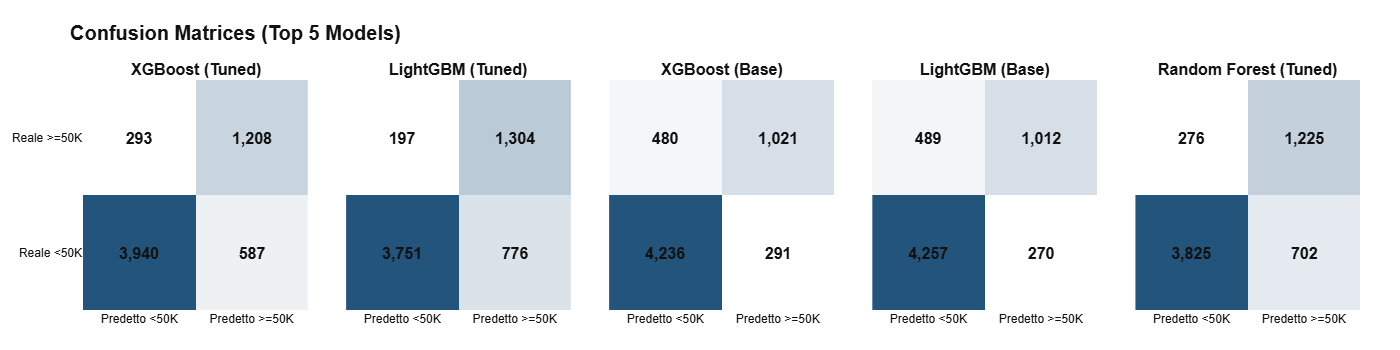
\includegraphics[width=\textwidth]{figures/matrice_confusione.png} 
    \caption{Confronto delle matrici di confusione per i modelli Top-5. Le celle diagonali (bianco e rosso scuro) rappresentano le classificazioni corrette.}
    \label{fig:matrice_confusione.png}
\end{figure}

\noindent
Il modello XGBoost Tuned mostra una robusta gestione della classe maggioritaria ($\le 50K$), minimizzando i Falsi Positivi. Tuttavia, si osserva un tasso fisiologico di Falsi Negativi (individui ad alto reddito classificati erroneamente come basso reddito), attribuibile alla sovrapposizione distributiva delle feature socio-demografiche nelle zone di confine decisionale.

\subsection{Metriche di Ranking (ROC e Precision-Recall)}

Poiché l'output primario del modello è uno score probabilistico $P(y=1|x)$, è fondamentale valutare la sua capacità di ordinare correttamente i casi positivi rispetto ai negativi, indipendentemente dalla soglia di classificazione.

\subsection{Curva ROC e AUC}
Tutti i modelli basati su Gradient Boosting mostrano prestazioni eccellenti, con un'Area Under Curve (AUC) superiore a $0.93$ (Tabella \ref{tab:auc_ranking}).
\begin{table}[H]
\centering
\begin{tabular}{lcc}
\toprule
\textbf{Modello} & \textbf{AUC-ROC} & \textbf{Rank} \\
\midrule
LightGBM (Tuned) & 0.9322 & 1 \\
XGBoost (Base) & 0.9319 & 2 \\
LightGBM (Base) & 0.9312 & 3 \\
\bottomrule
\end{tabular}
\caption{Ranking basato su AUC. Le differenze tra i primi tre modelli sono marginali ($<0.001$), indicando una sostanziale equivalenza nel potere discriminante.}
\label{tab:auc_ranking}
\end{table}


\begin{figure}[H]
    \centering
    % Placeholder per l'immagine Plotly (Matrici di Confusione)
    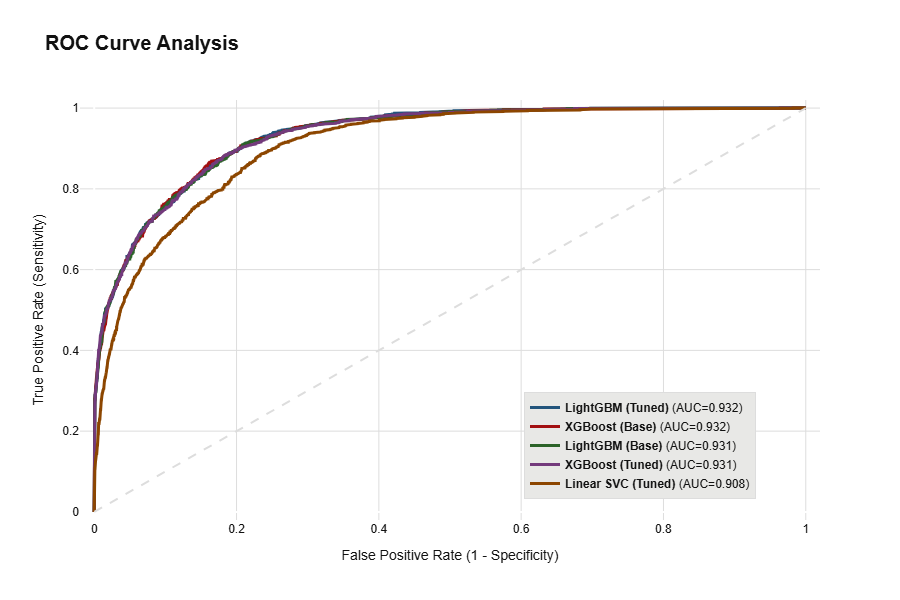
\includegraphics[width=\textwidth]{figures/roc.png} 
    \caption{AUC-ROC dei 5 modelli più performati con LightGBM (Tuned) e XGBoost (Base) valutaticome i migliori}
    \label{fig:roc.png}
\end{figure}

\subsection{Precision-Recall (PR) Curve}
In contesti sbilanciati, l'Average Precision (AP) è una metrica più informativa dell'AUC. LightGBM (Tuned) domina questa classifica con un AP di \textbf{0.8427}, dimostrando una superiorità nel mantenere alta la precisione anche a livelli elevati di recall, una caratteristica cruciale per minimizzare i falsi allarmi.


\begin{figure}[H]
    \centering
    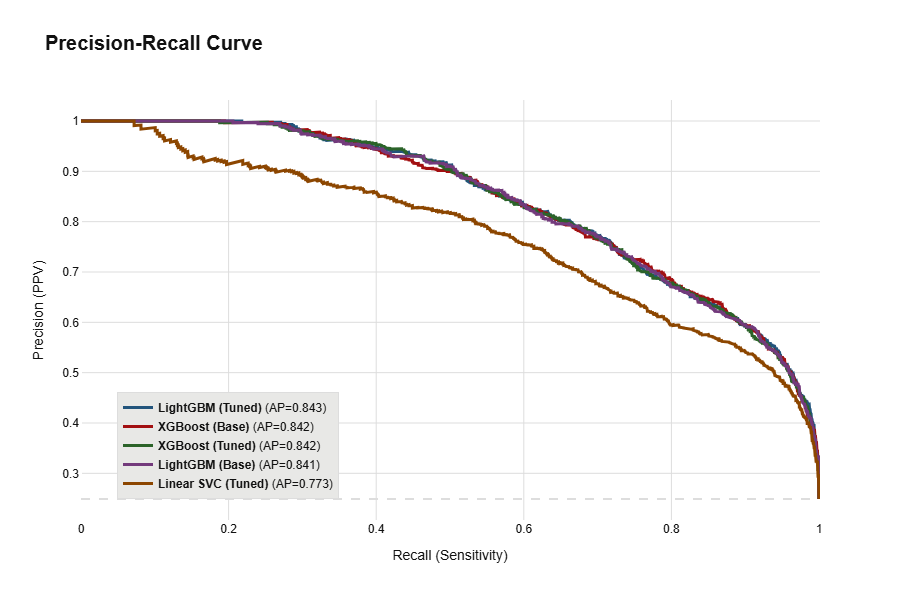
\includegraphics[width=\textwidth]{figures/prc.png} 
    \caption{Il confronto tra i modelli mostra prestazioni molto simili per LightGBM e XGBoost ($AP \approx 0.84$), che mantengono valori di precision elevati lungo gran parte del range di recall. Il Linear SVC presenta invece performance inferiori (AP = 0.773), con una diminuzione più marcata della precision all’aumentare della recall.}
    \label{fig:prc.png}
\end{figure}

\subsection{Analisi di Calibrazione (Reliability)}

Un modello è "ben calibrato" se la probabilità predetta riflette la frequenza empirica dell'evento (e.g., tra tutti i casi predetti con probabilità 0.7, il 70\% dovrebbe essere effettivamente positivo).
L'analisi mediante \textit{Calibration Plot} e \textbf{Brier Score} (Tabella \ref{tab:calibration}) conferma l'eccellenza di LightGBM.

\begin{table}[h]
\centering
\begin{tabular}{lcc}
\toprule
\textbf{Modello} & \textbf{Brier Score} (Lower is better) & \textbf{Rank} \\
\midrule
\textbf{LightGBM (Tuned)} & \textbf{0.0876} & \textbf{1} \\
CatBoost (Tuned) & 0.0878 & 2 \\
XGBoost (Tuned) & 0.0880 & 3 \\
\bottomrule
\end{tabular}
\caption{Valutazione della calibrazione probabilistica. LighXGBoost (Base) ottiene il punteggio Brier più basso, indicando stime di probabilità altamente affidabili.}
\label{tab:calibration}
\end{table}

\noindent
Il basso Brier Score (0.0876) indica che XGBoost (Base) produce probabilità predittive complessivamente accurate e ben calibrate. Pertanto, le stime possono essere utilizzate per decisioni di business (es. risk scoring), pur potendo valutare eventuali tecniche di ricalibrazione per ulteriori miglioramenti.

\subsection{Comparazione Grafica della Calibrazione}

A completamento della validazione statistica, il modello \textit{Champion} e i principali competitor sono stati sottoposti a una diagnostica strutturale volta a valutarne l'efficienza computazionale, i driver decisionali e la stabilità rispetto al rischio di overfitting.

\begin{figure}[H]
    \centering
    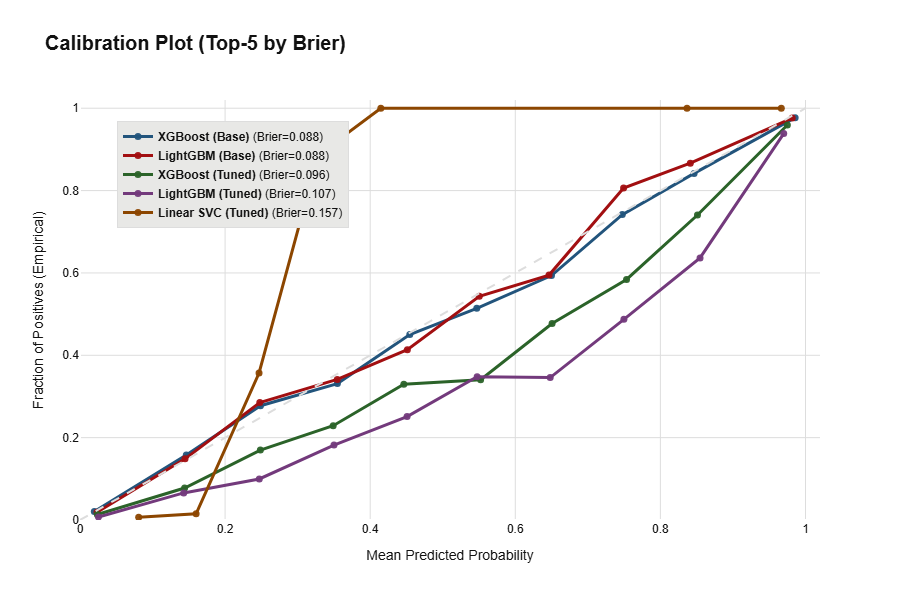
\includegraphics[width=\textwidth]{figures/calibration.png} 
    \caption{I modelli XGBoost e LightGBM nella versione base mostrano la calibrazione migliore ($Brier \approx 0.088$), con curve vicine alla diagonale ideale. Le versioni tuned presentano una calibrazione leggermente peggiore, mentre Linear SVC evidenzia la performance più bassa ($Brier \approx 0.157$).}
    \label{fig:calibration.png}
\end{figure}

\subsection{Frontiera di Efficienza (Time-Accuracy Trade-off)}

L'analisi comparativa dei costi computazionali (Tabella \ref{tab:efficiency}) evidenzia differenti profili di utilizzo risorse.
Sebbene \textbf{Linear SVC (Tuned)} risulti l'algoritmo più rapido in fase di inferenza (\(t_{inf} \approx 67\)ms), il modello selezionato \textbf{XGBoost (Tuned)} offre un compromesso globale accettabile, garantendo il massimo F1-Score (0.7330) con un tempo di latenza ampiamente contenuto (\(t_{inf} \approx 114\)ms), pienamente compatibile con requisiti di batch scoring o real-time moderato.

\begin{table}[H]
\centering
\begin{tabular}{lcc}
\toprule
\textbf{Modello} & \textbf{Latenza Inferenza (s)} & \textbf{F1-Score} \\
\midrule
Linear SVC (Tuned) & 0.0667 & 0.6840 \\
LightGBM (Base) & 0.0914 & 0.7273 \\
XGBoost (Base) & 0.1121 & 0.7259 \\
\textbf{XGBoost (Tuned)} & \textbf{0.1135} & \textbf{0.7330} \\
LightGBM (Tuned) & 0.2313 & 0.7283 \\
\bottomrule
\end{tabular}
\caption{Analisi trade-off efficienza/efficacia. le performances predittive con un overhead computazionale accettabile.}
\label{tab:efficiency}
\end{table}

\begin{figure}[H]
    \centering
    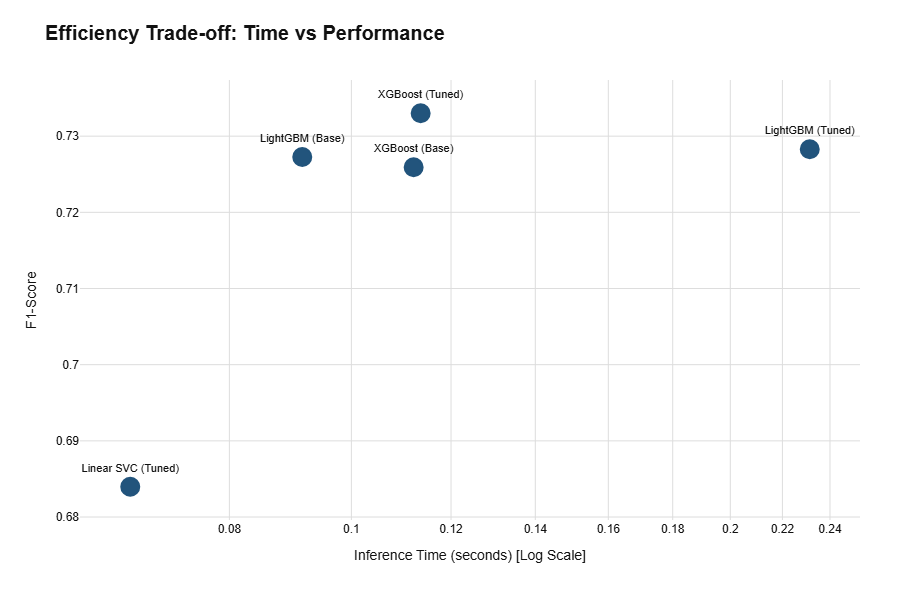
\includegraphics[width=\textwidth]{figures/time.png} 
    \caption{Il grafico mostra comem si distribuiscono i modelli nella loro performance di addestramento in relazione al tempoimpiegato.}
    \label{fig:time.png}
\end{figure}


\subsection{Feature Importance e Interpretabilità Globale}

Per comprendere i driver latenti del processo decisionale, è stata estratta la classifica delle feature. L'analisi per il modello vincitore \textbf{XGBoost (Tuned)} (Figura \ref{fig:FI_X.png}) si basa sull'importanza calcolata tramite il parametro \textit{Gain} (la riduzione dell'impurità media apportata da ciascuna variabile) e rivela una struttura gerarchica molto chiara:

\begin{enumerate}
    \item \textbf{Dominanza dello Stato Civile e Relazioni:} La variabile dummy \texttt{marital.status\_Married-civ-spouse} risulta di gran lunga il discriminante principale (con un Gain di circa 0.32), seguita da altre variabili relazionali come \texttt{relationship\_Husband}. Questo indica che la stabilità familiare e la probabilità di un doppio reddito aggregato costituiscono il fattore più predittivo per il superamento della soglia dei 50K.
    \item \textbf{Capitale Finanziario:} \texttt{capital.gain} emerge come il secondo driver più forte in assoluto, confermando che l'accumulazione di ricchezza tramite investimenti finanziari diretti è un indicatore inequivocabile di reddito elevato.
    \item \textbf{Istruzione e Professione:} \texttt{education.num} mantiene un peso cruciale nel modello, supportando la teoria del capitale economico legato alle competenze. Parallelamente emergono categorie professionali ad alto reddito come \texttt{occupation\_Exec-managerial}.
\end{enumerate}

\noindent
Al contrario, osservando le metriche estratte da \textbf{LightGBM} (Figura \ref{fig:FI_L.png}), si nota una predilezione netta per le variabili continue (\texttt{age}, \texttt{hours.per.week}). Questo comportamento è tipico quando l'importanza viene misurata in base alla metrica di \textit{Split} (frequenza di taglio nei rami dell'albero), che tende fisiologicamente a premiare le variabili ad alta cardinalità rispetto alle categoriche, offrendo molteplici punti di segmentazione. Entrambe le gerarchie, seppur calcolate in modo diverso, validano la plausibilità semantica e le aspettative di dominio economico dell'esperimento.

\begin{figure}[H]
    \centering
    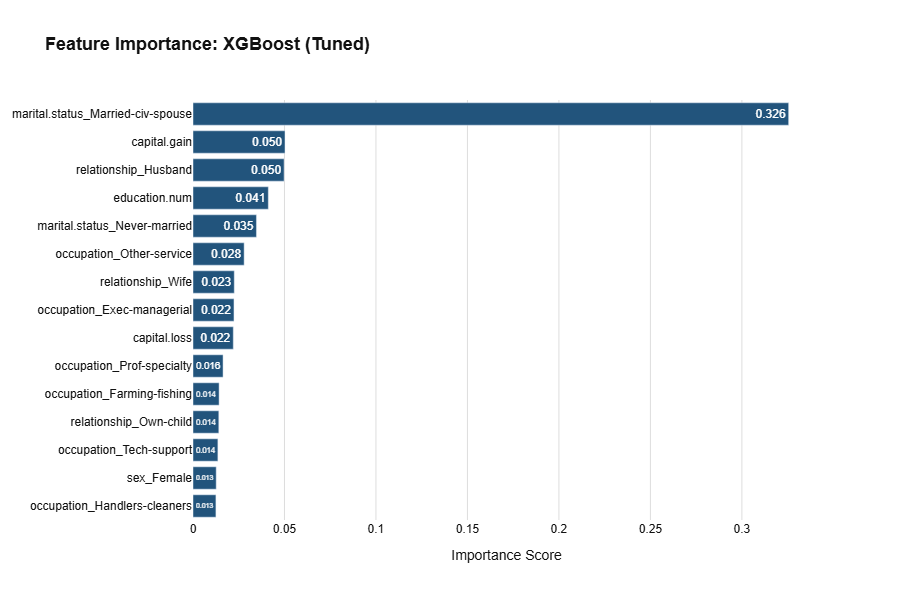
\includegraphics[width=\textwidth]{figures/FI_X.png} 
    \caption{Importanza delle feature per il modello XGBoost (Tuned), misurata tramite Gain. Lo stato civile domina nettamente la capacità predittiva.}
    \label{fig:FI_X.png}
\end{figure}

\begin{figure}[H]
    \centering
    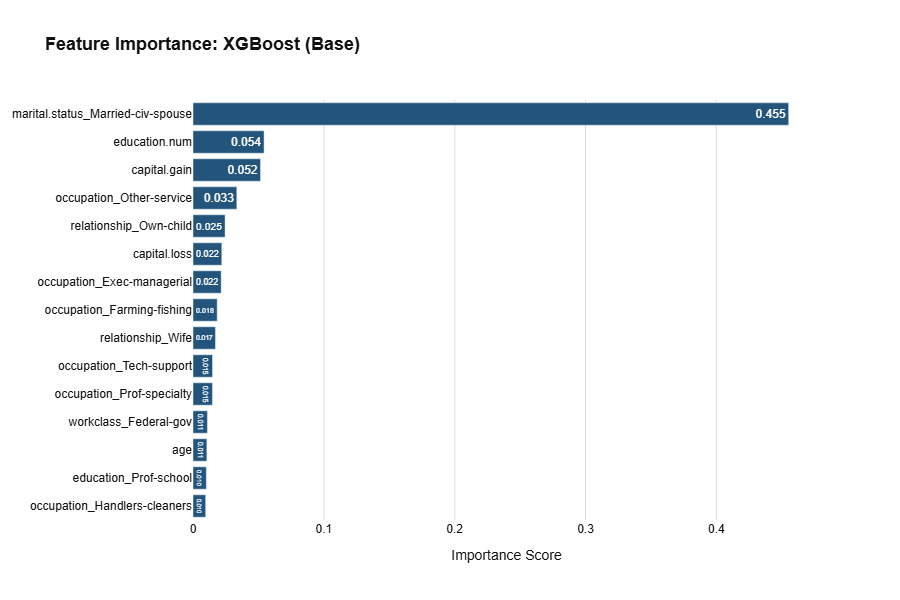
\includegraphics[width=\textwidth]{figures/FI_XB.png} 
    \caption{Importanza delle feature per il modello XGBoost (Base).}
    \label{fig:FI_XB.png}
\end{figure}

\begin{figure}[H]
    \centering
    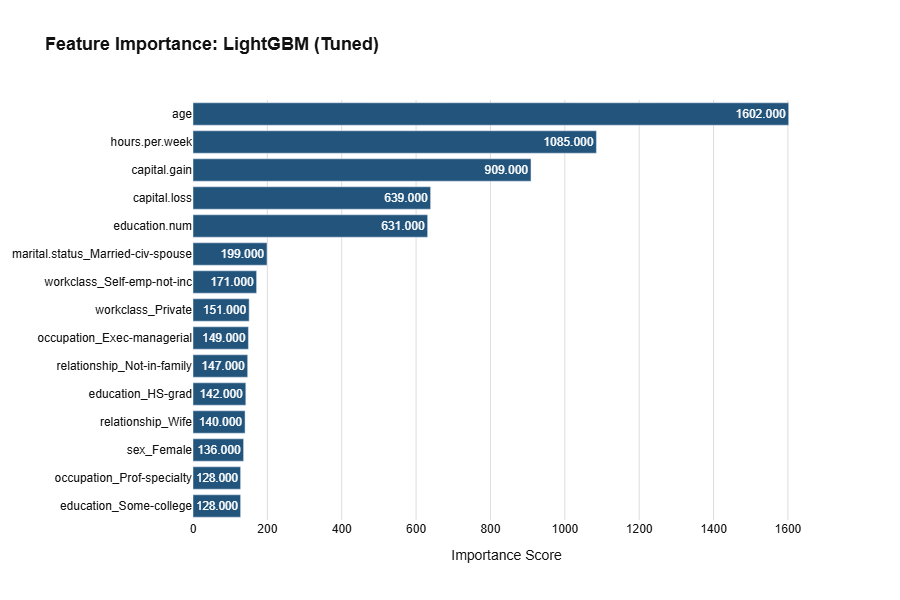
\includegraphics[width=\textwidth]{figures/FI_L.png} 
    \caption{Importanza delle feature per il modello LightGBM (Tuned). A differenza di XGBoost, le variabili continue dominano la classifica a causa dell'impatto della metrica di conteggio degli split.}
    \label{fig:FI_L.png}
\end{figure}

\begin{figure}[H]
    \centering
    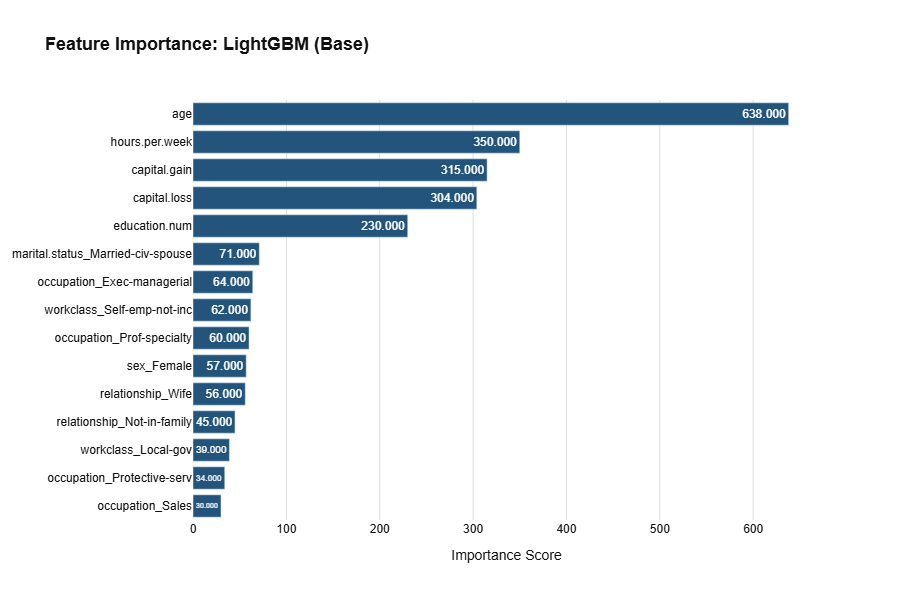
\includegraphics[width=\textwidth]{figures/FI_LB.png} 
    \caption{Importanza delle feature per il modello LightGBM (Base).}
    \label{fig:FI_LB.png}
\end{figure}


\section{Analisi del Rischio di Overfitting (Generalization Gap)}

La stabilità della generalizzazione è stata quantificata misurando il \textit{Gap} tra l'accuratezza sul set di training (\(Acc_{train}\)) e quella sul set di test (\(Acc_{test}\)). Un gap ridotto è indice di un modello che apprende pattern robusti senza memorizzare il rumore statistico del campione di addestramento.

\begin{table}[h]
\centering
\begin{tabular}{lccc}
\toprule
\textbf{Modello} & \textbf{Acc. Train} & \textbf{Acc. Test} & \textbf{Gap (\(\Delta\))} \\
\midrule
Linear SVC (Tuned) & 0.8026 & 0.8021 & 0.0005 \\
LightGBM (Base) & 0.8832 & 0.8741 & 0.0091 \\
LightGBM (Tuned) & 0.8565 & 0.8386 & 0.0179 \\
XGBoost (Base) & 0.8924 & 0.8721 & 0.0203 \\
\textbf{XGBoost (Tuned)} & \textbf{0.8779} & \textbf{0.8540} & \textbf{0.0239} \\
\bottomrule
\end{tabular}
\caption{Analisi del Generalization Gap. Tutti i modelli mostrano un rischio di overfitting "Basso" (\(\Delta \le 0.05\)).}
\label{tab:overfitting_gap}
\end{table}

\noindent
I risultati (Tabella \ref{tab:overfitting_gap}) dimostrano l'efficacia delle tecniche di regolarizzazione impiegate. Modelli lineari più semplici come la \textbf{Linear SVC} presentano fisiologicamente un gap pressoché nullo (\(0.05\%\)), a fronte però di un potere predittivo inferiore. Il modello vincitore \textbf{XGBoost (Tuned)} mantiene un gap decisamente contenuto (\(\approx 2.4\%\)), significativamente inferiore alla soglia di attenzione del 5\%. Questo garantisce che le prestazioni osservate in fase di test siano una stima affidabile e solida del comportamento futuro del modello in un ambiente di produzione.

\begin{figure}[H]
    \centering
    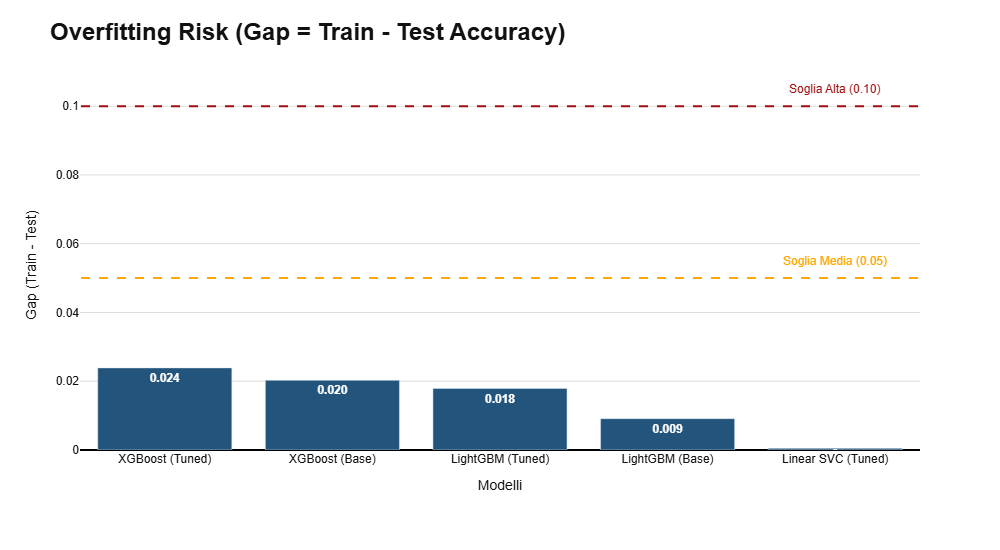
\includegraphics[width=\textwidth]{figures/overfitting.png} 
    \caption{Confronto delle accuratezze in fase di addestramento e di test. Il divario ridotto (Gap) conferma una generalizzazione stabile e un basso rischio di overfitting per tutti i modelli selezionati.}
    \label{fig:overfitting.png}
\end{figure}

\end{appendices}

\end{document}

